
\begin{document}

\chapter{Planner Methodology}

\label{chapter:methodology}

As described briefly in Sec.~\ref{sec:finaldesign}, the final planner design
uses a probabilistic roadmap to capture the connectivity of the environment and
uses a novel variant of best first search to find a safe, low cost path the
goal. This approach is called Dodger. This section describes the algorithm as
well as formalizes the definition of a dynamic obstacle and its associated cost
distribution and motion.

\section{Dynamic Obstacles}

As a major component of this work, dynamic obstacles need to be designed such
that one can describe their trajectories, initial configurations, and their
levels of uncertainty. This section introduces the definition of a dynamic
obstacle used throughout this work along with how one is represented to the
planner and its simulated \& predicted equations of motion. Specifically, the
formal definition of a dynamic obstacle will be introduced, a novel way of
representing obstacles using a cost distribution will be formalized, and their
predicted and simulated motion will be described.

\subsection{Definition}

\label{sec:def}

A dynamic obstacle is defined as a 5-tuple, $a = (I, \dot{\zeta},
\epsilon, \xi, T)$ where $I$ is the initial configuration of the obstacle,
$\dot{\zeta}$ is a function, $\dot{\zeta}: \mathbb{R}^+ \rightarrow
\mathbb{R}^2$, representing the velocity of the obstacle, $\epsilon$ is used to
define a random variable $\rho \sim \mathcal{U}(-\epsilon, \epsilon)$ that is
used to inject noise into an obstacle's trajectory shown in
Eq.~\ref{eq:obs_observed} where $\mathcal{U}$ is a uniform distribution, $\xi$
is the current configuration used for prediction, and $T$ is the time that the
obstacle was in configuration $\xi$.  The variables $\xi$ and $T$ are dynamic
variables and are updated throughout the execution of the algorithm and are
used to determine when it is appropriate for the algorithm replan and find a
new path through the environment using more up to date information. This is
explained in Sec.~\ref{sec:design_planner}. The variables $\xi$ and $T$ are
initially set to $I$ and $0$ respectively. It is assumed that the robot has
access to this information about the dynamic obstacles and will use it to
safely around them.  Information such as the initial configuration and the
velocity equation for each dynamic obstacle are assumed to be determined by an
external system that is either using a machine learning technique to deduce
these properties by using information about where the dynamic obstacle has been
before or by an external planning system such as in a warehouse that is
commanding the velocities and configurations of these dynamic obstacles. This
is the same assumption as that made by Phillips et al~\cite{sipp} and Narayanan
et al~\cite{asipp}.

\subsection{Cost Distribution}

\label{sec:cost}

Unlike in the previous work, dynamic obstacles are represented by cost
distributions that resemble probability density functions. The difference being
is that these cost distributions do not have a unit integral. These cost
distributions are used to describe where the obstacle is going to be in within
a time interval and can be generated by a third party system, such as a motion
capture system. There is an assumption that for a given interval, $\mathcal{T}
= [t_0, t_m]$, the highest cost with the smallest uncertainty will be at $t =
t_0$ and the lowest cost with the highest uncertainty will be at $t = t_m$.
Under this assumption, the cost function models how the obstacle may diverge
from its current trajectory as time increases. With these assumptions, the cost
function, $P_a: \mathbb{R}^2 \times (\mathbb{R}^+)^2 \rightarrow
\mathbb{R}$, represents represents the cost surface for a given dynamic
obstacle, $a$,  within a given time interval. Eq.~\ref{eq:singleprob} formally
defines the cost function for a single obstacle.

% Single agent PDF

\begin{equation}
    P_a(x, y, t_0, t_m) = \frac{1}{t_m} \cdot \int^{t_m}_{t_0}
    \mathcal{N}(\zeta_a(t), \alpha \cdot (t - t_0)^2 + \beta, x, y) \cdot
    (t_m - t)^{\gamma} \,\mathrm{d}t
    \label{eq:singleprob}
\end{equation}

In Eq.~\ref{eq:singleprob}, $\mathcal{N}(\mu, \sigma^2, x, y)$ is the
evaluation of a 3D normal distribution centered at $(\mu_x, \mu_y)$ with a
variance of $\sigma^2$ at $(x, y)$ and $\alpha$, $\beta$, and $\gamma$ are
scaling constants such that $\alpha > 0$, $\beta > 0$, and $\gamma \geq 1$.
Fig.~\ref{fig:normal_3d} shows an example of $\mathcal{N}$. The normal
distribution works as a basis function to describe the possible trajectories of
the dynamic obstacle. This equation models how the uncertainty of obstacle
trajectory prediction increases over time by increasing the standard deviation
of the Gaussian distribution as the time increases.  Likewise, this function
multiplies the Gaussian distribution by a factor of $(t_m - t)^{\gamma}$ where
$\gamma \geq 1$ which gives higher costs to times closer to $t_0$.

\begin{figure}[h!]
    \centering
    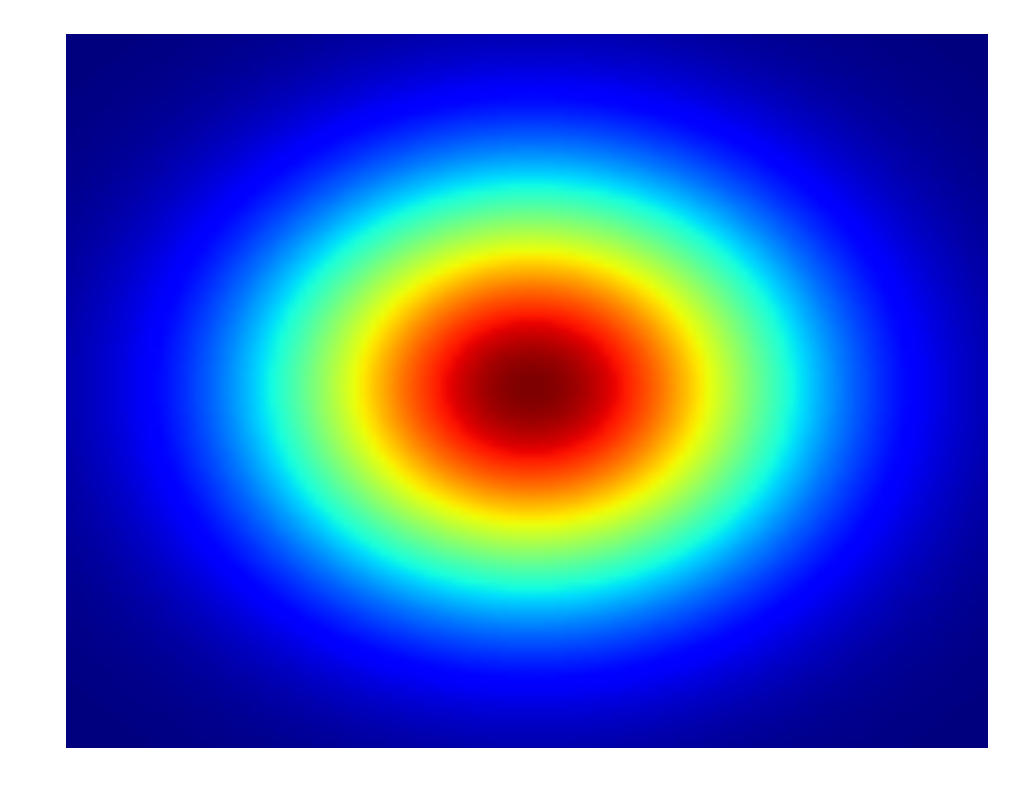
\includegraphics[width=0.60\linewidth]{figs/normal_3d}

    \caption{A plot depicting the three dimensional normal distribution
    $\mathcal{N}(\cdot)$ that is used as a basis function for the obstacle cost
distribution. The more red an area, the higher the cost. The more blue an area,
the lower the cost.}

    \label{fig:normal_3d}
\end{figure}

A cost function is also needed that can incorporate the cost distributions for
multiple dynamic obstacles within the environment. The cost function used in
this work, $P: \mathbb{R}^2 \times (\mathbb{R}^+)^2 \times \mathcal{A}
\rightarrow \mathbb{R}$ where $\mathcal{A}$ is the set of all possible sets of
dynamic obstacles, calculates the average cost at a point $(x, y)$ within a
given time interval for a given set of dynamic obstacles, $A$. This is shown
formally in Eq.~\ref{eq:prob}.

% Multiple agent PDF

\begin{equation}
    P(x, y, t_0, t_m, A) = \frac{\mathlarger{\sum_{a \in A} P_a(x, y, t_0,
    t_m)}}{|A|}
    \label{eq:prob}
\end{equation}

An example of how $P$ changes over time is shown in Fig.~\ref{fig:agent_cost}.
In that example, two dynamic obstacles are placed in the scene and given
sinusoidal velocities. In this example the time interval, $\delta t$, is kept
constant throughout the simulation, i.e. $t_m = t_0 + \delta t$, for all $t_0
\in [0, T - \delta t]$ where $T$ is the length of the simulation. Since the
velocity does not remain constant in the example, the cost distribution
elongates an shrinks based on the acceleration of the obstacle. For instance,
in the first and last images in Fig.~\ref{fig:agent_cost}, the cost is
contained to a small area due to the velocity equations of the obstacles being
at their minimum and in the fourth image,the cost is more spread out through
the environment because the velocity is at its maximum.

\begin{figure}[h!]

    \centering

    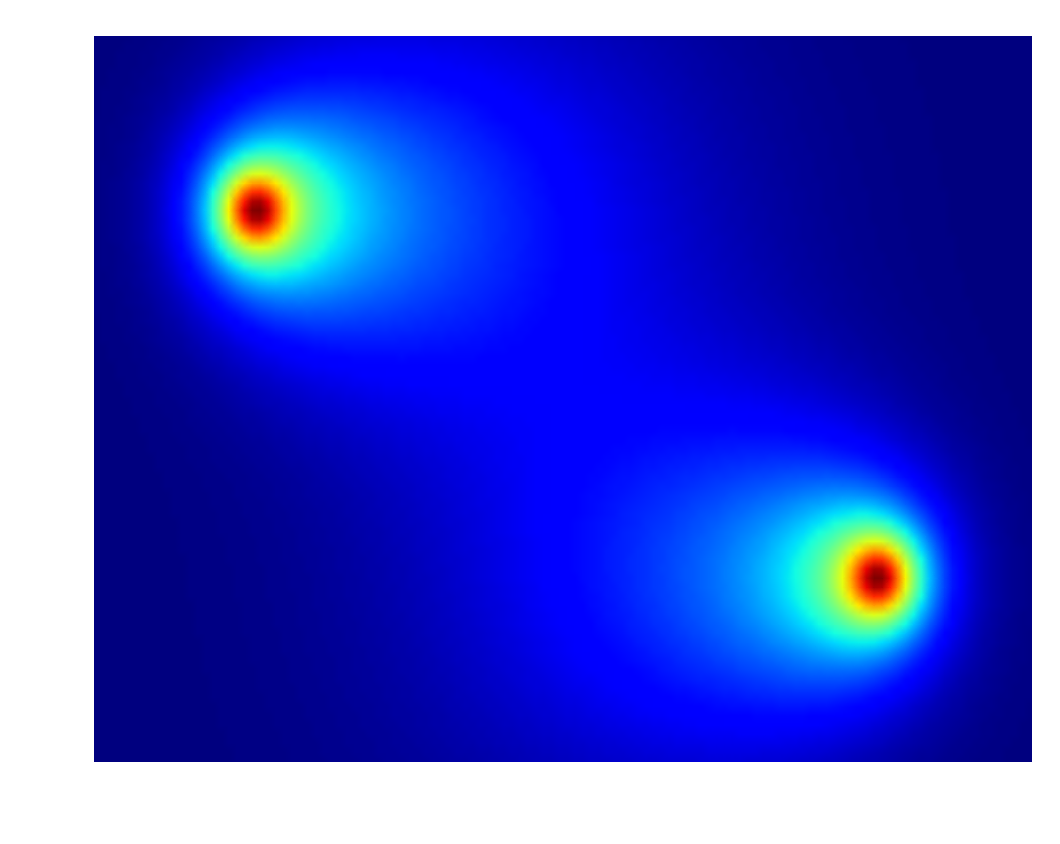
\includegraphics[width=0.24\linewidth]{figs/agent_1}
    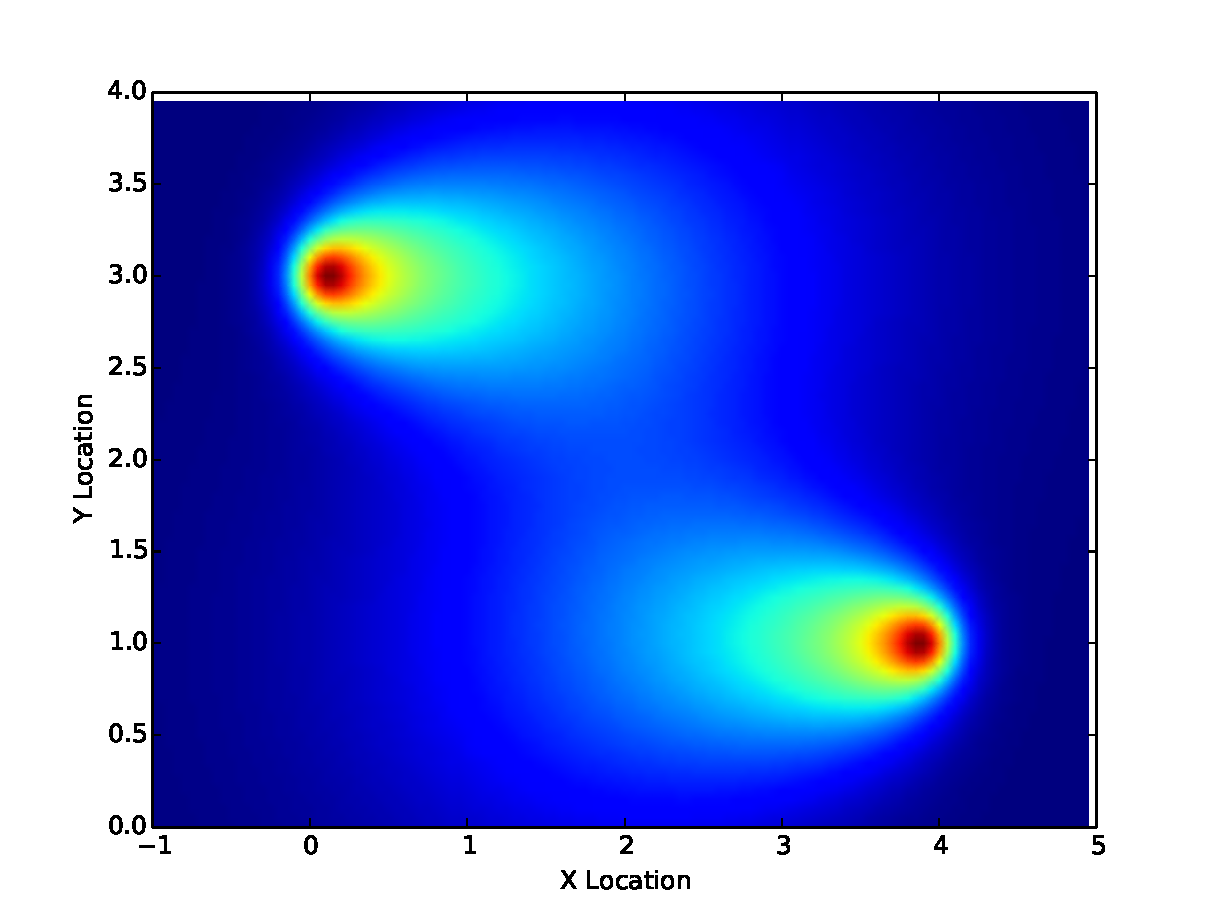
\includegraphics[width=0.24\linewidth]{figs/agent_2}
    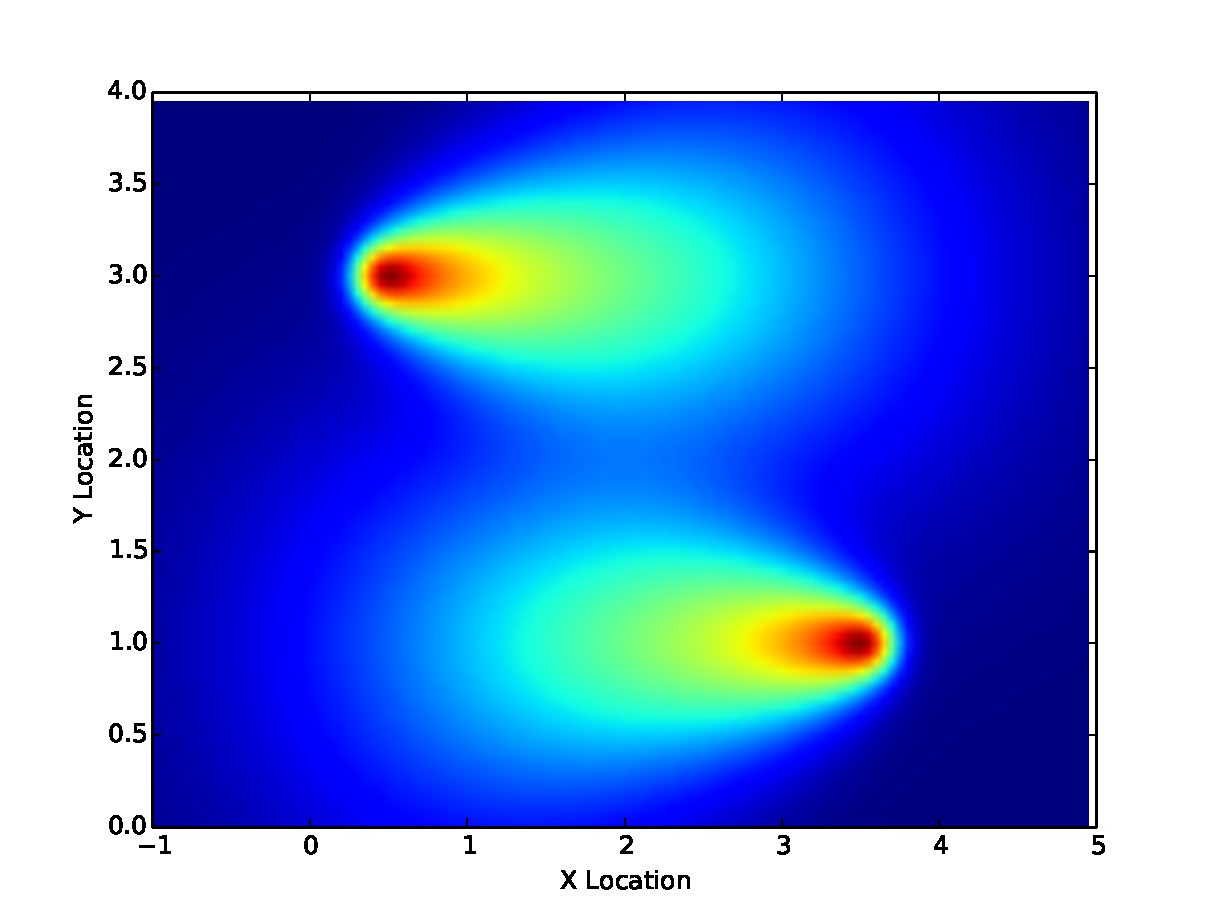
\includegraphics[width=0.24\linewidth]{figs/agent_3}
    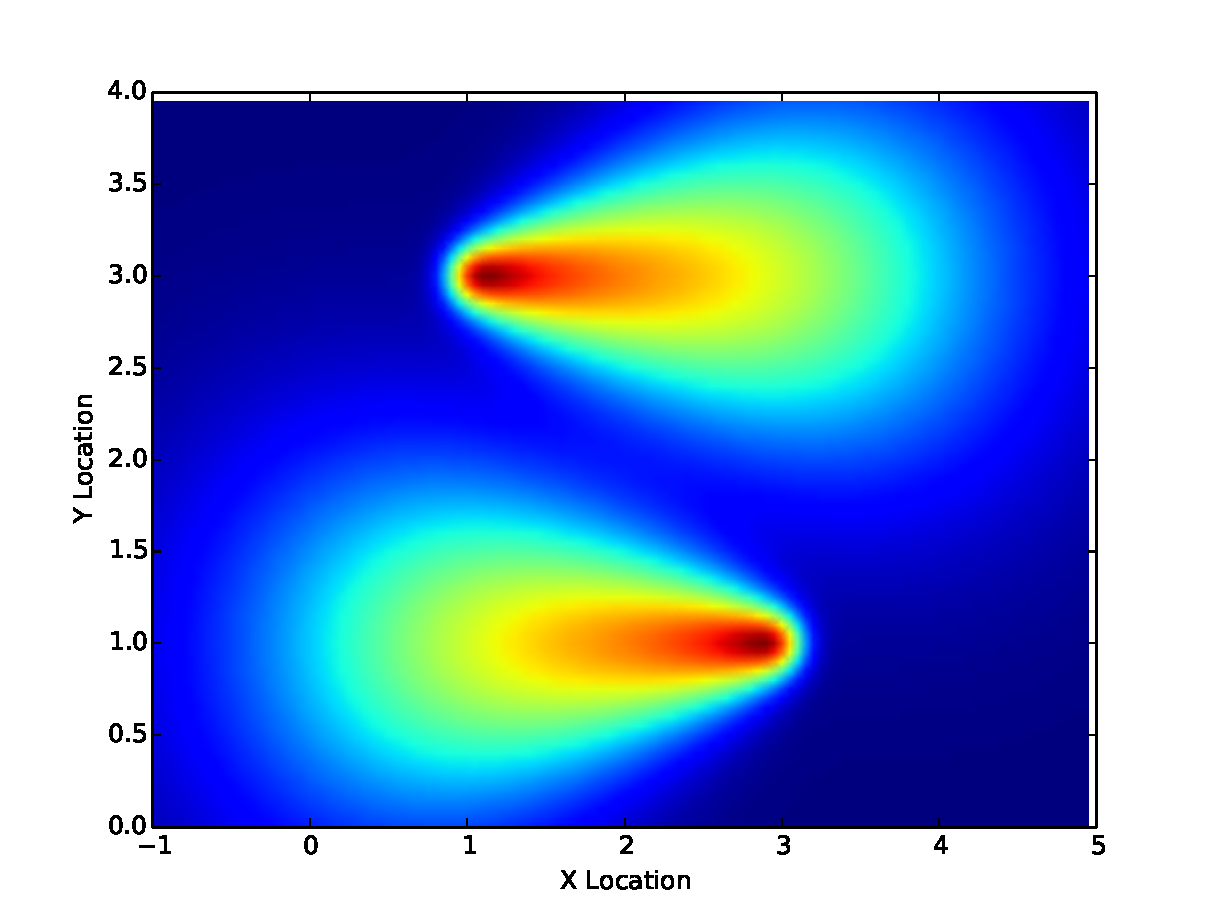
\includegraphics[width=0.24\linewidth]{figs/agent_4} \\
    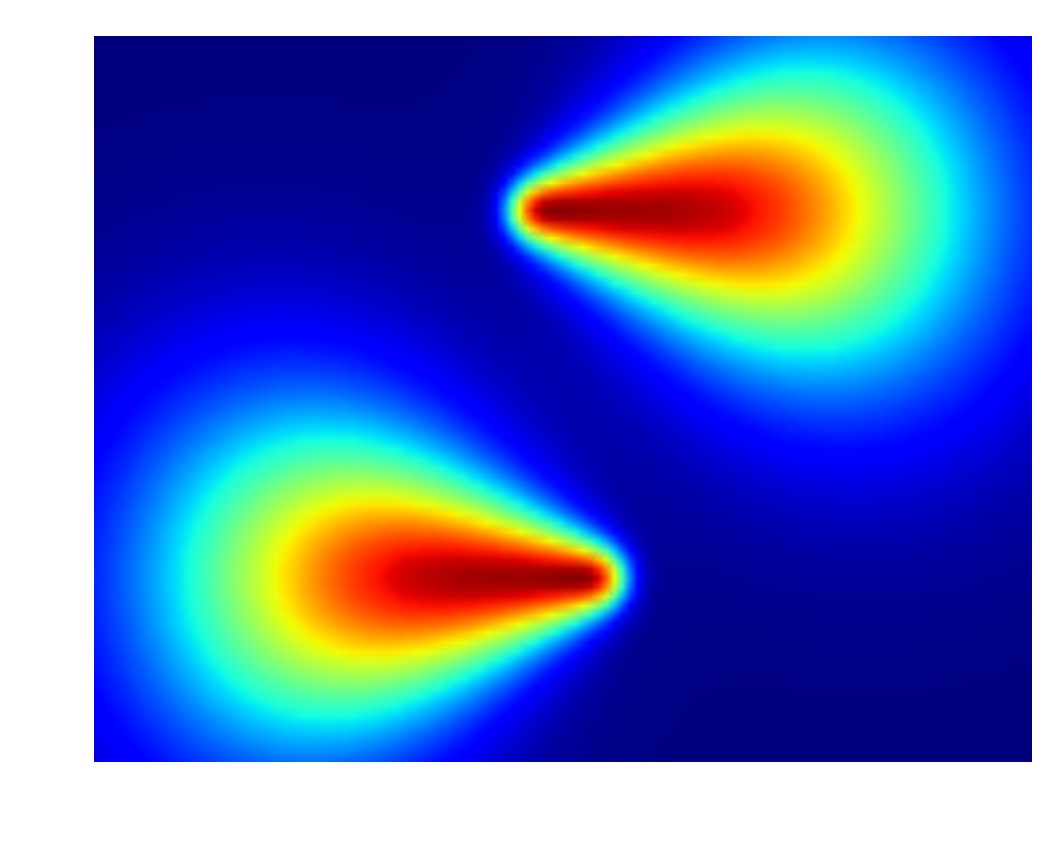
\includegraphics[width=0.24\linewidth]{figs/agent_5}
    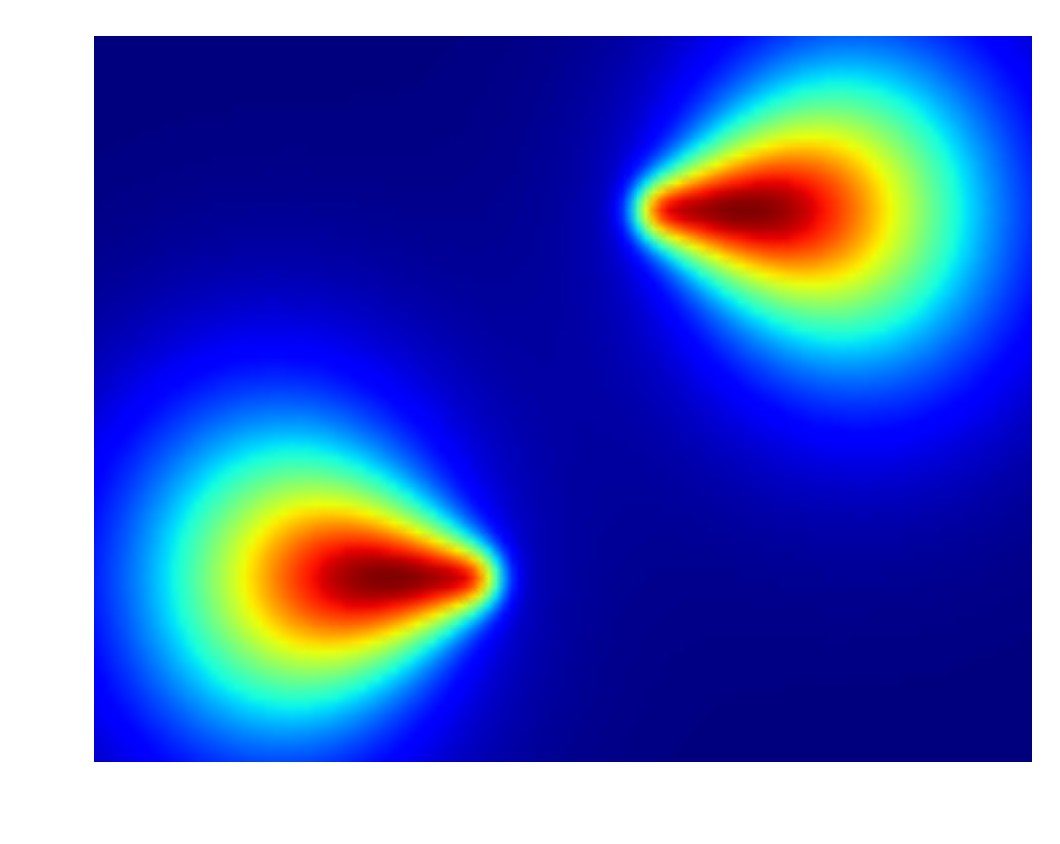
\includegraphics[width=0.24\linewidth]{figs/agent_6}
    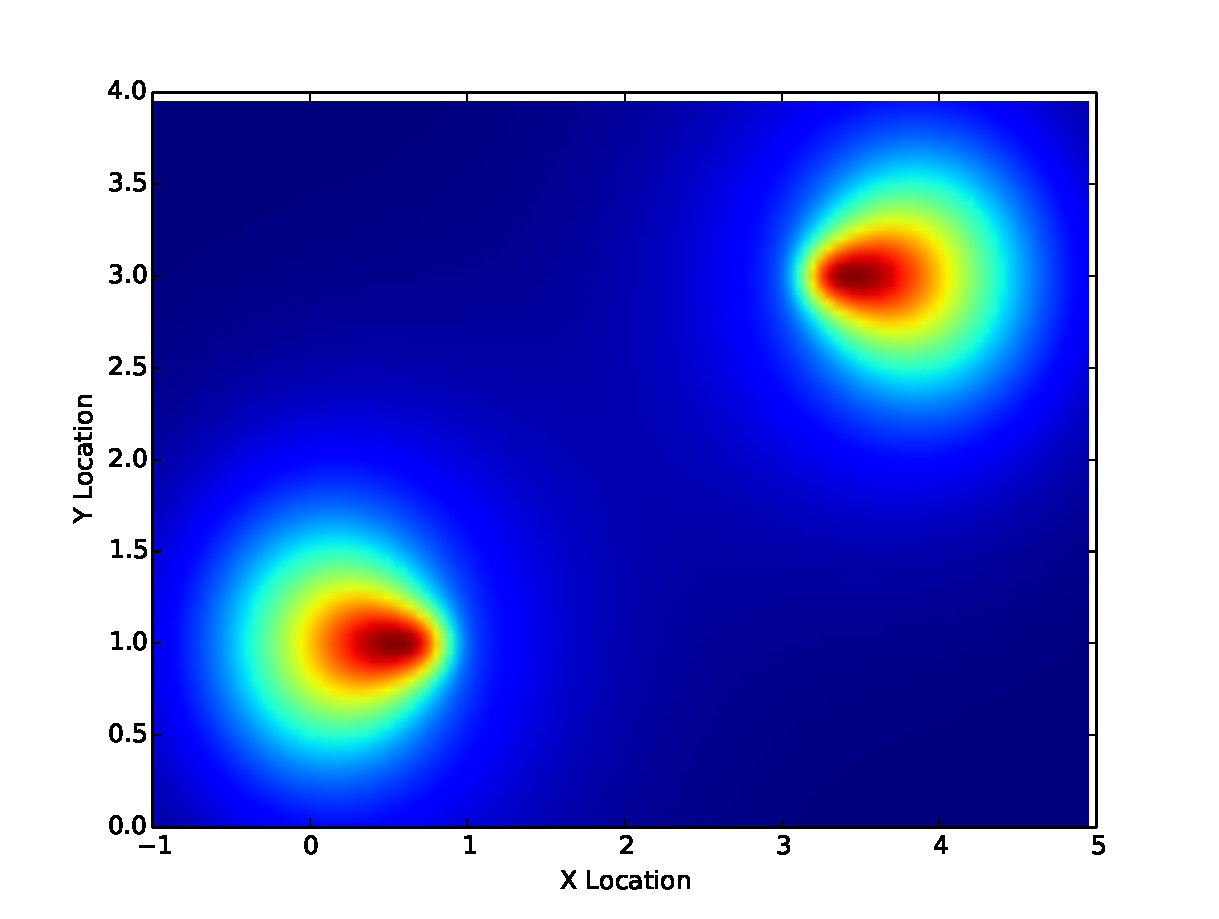
\includegraphics[width=0.24\linewidth]{figs/agent_7}
    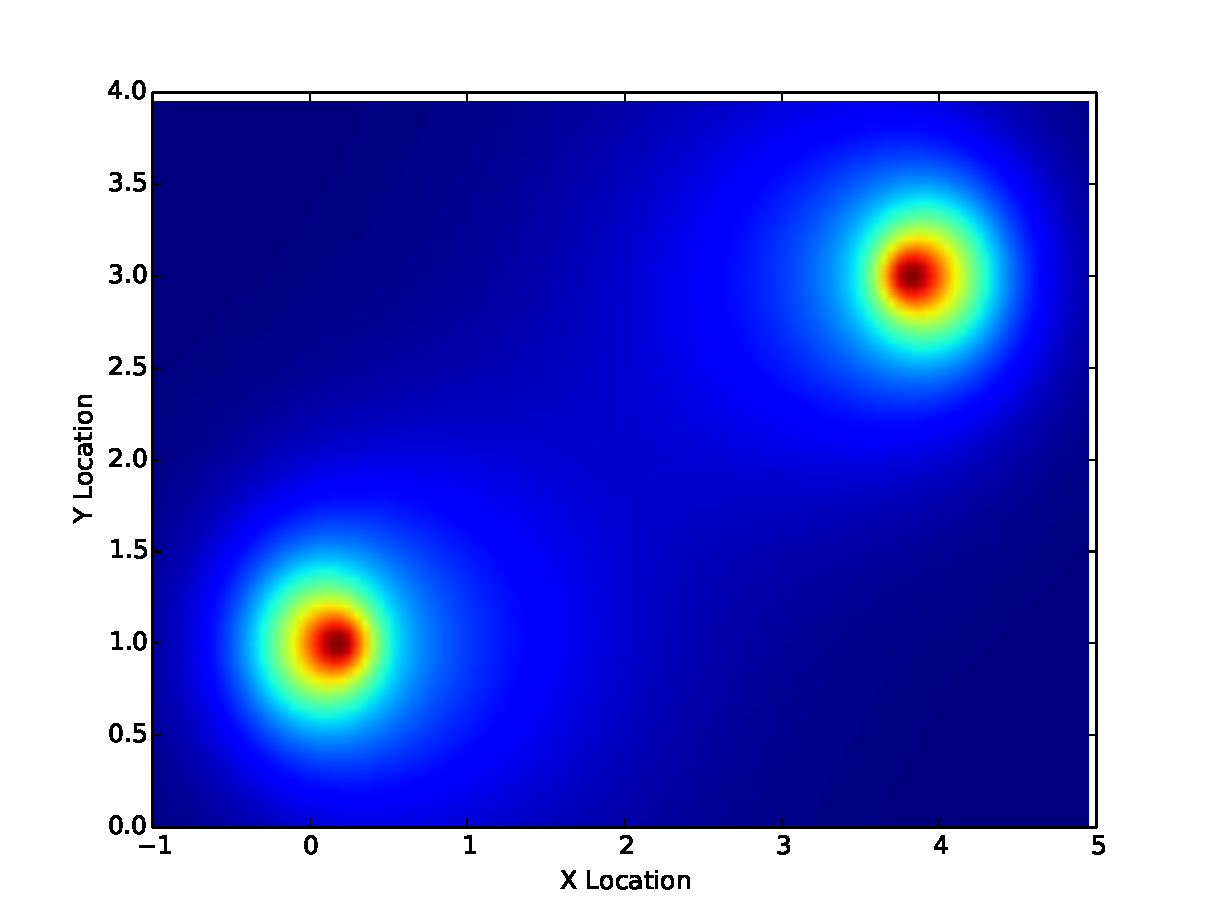
\includegraphics[width=0.24\linewidth]{figs/agent_8}

    \caption{Cost distributions indicating the likelihood that a dynamic
    obstacle will be at a certain location within a given time interval. These
figures show how this distribution changes over time. The sequence progress
from left to right, top to bottom}

    \label{fig:agent_cost}

\end{figure}

\subsection{Equations of Motion}

\label{sec:motion}

The motion of a dynamic obstacle is defined by the velocity equation, the
initial configuration, the amount of uncertainty. Defining the obstacle's
trajectory in terms of its velocity makes it easier to model when creating
scenes. The equation of motion for the dynamic obstacle is shown in
Eq.~\ref{eq:obs_pred}.

\begin{equation}
    \zeta_a(t) =
        \begin{cases}
            \xi_a + \mathlarger{\int_{T_a}^{t}} \dot{\zeta_a}(\lambda) \,
            \mathrm{d}\lambda
            & \text{if } t \geq T_a \\
            \tilde{\zeta_a}(t) & \text{if } t < T_a
        \end{cases}
    \label{eq:obs_pred}
\end{equation}

In Eq.~\ref{eq:obs_pred}, $\tilde{\zeta_a}$ represents the observed trajectory
of the obstacle whereas $\zeta_a$ corresponds to the predicted trajectory of
the obstacle. This disambiguation is needed because the planner needs to be
able to extrapolate the future movements of a dynamic obstacle. The variables,
$\xi_a$ and $T_a$ are dynamically updated when the planner replans and are
initially set to $I_a$ and $0$ respectively. The need for this and how it is
designed will be discussed in Sec.~\ref{sec:design_planner}

For the experiments, the motion of the obstacles is simulated by adding a
random variable, $\rho \sim \mathcal{U}(-\epsilon, \epsilon)$ to the trajectory
during the numerical integration of the velocity equation. This form of
stochasticity allows the obstacle to diverge from its specified trajectory
whilst maintaining the same velocity equation. This means that the obstacle
will not exhibit random, Brownian motion around its specified path, but rather
is able to diverge completely. Also, by adding the random variable to the
velocity equation during the numerical integration, the obstacle will not
"jump" to a new location, but will gradually diverge off of its specified path.
The definition of $\tilde{\zeta_a}$ is shown in Eq.~\ref{eq:obs_observed}.  For
this equation, it is assumed that the function only computes a value for any
given time value, $t$, only once.

\begin{equation}
    \tilde{\zeta_a}(t) =
        \begin{cases}
            \tilde{\zeta_a}(t - \delta t) + \dot{\zeta_a}(t) \cdot \delta t
            + \rho
            & \text{if } t > 0 \\
            I_a & \text{if } t = 0
        \end{cases}
    \label{eq:obs_observed}
\end{equation}

In Eq.~\ref{eq:obs_observed}, $\delta t$ is a constant where $\delta t > 0$ and
is used for the numerical integration of the velocity. Numerical integration is
used in order to allow the path to diverge. Since a recursive function is used
for determining the current position of the obstacle, the obstacle's next
location will be determined by its last location, its velocity, and a certain
error factor $\rho$. This will allow the obstacle to exhibit more than simply
Brownian motion along a path and it will be able to diverge completely from its
specified path. This type of uncertainty is important because it is exhibited
in real-world scenarios such as error propagation in controls and by simply not
having enough information about the actual velocity equation for a given
obstacle. The full extent of $\tilde{\zeta_a}$ is not known by the planner and
this equation is only used to simulate the motion of the obstacles for
experimentation and evaluation of the developed planner.

By increasing the level of stochasticity, $\epsilon$, for a given dynamic
obstacle, it will be more likely to diverge from its current path. This means
that the uncertainty of a given dynamic obstacle can be parametrized by its
value for $\epsilon$.

The motion of a dynamic obstacle is described by it's velocity and a starting
location in order for the planner to be able to continue to predict an
obstacle's motion even when it diverges from its current path. If the
obstacle's motion was described by parametric equations of its position, it
would not be possible to continue to predict where it is going to move once it
is no longer following its prescribed path since the obstacle may diverge from
this path completely.

\subsection{Available Information}

It is important to note what information is available to the planner. It is not
assumed that the planner has perfect information about the motion of the
obstacles or their associated definitions. The planner only has access to the
obstacles' velocity equations and their positions throughout the execution of
path.  The planner does not know the amount of noise, $\epsilon$, being
injected into the obstacles' velocities as described in Sec.~\ref{sec:motion}.
It is also assumed that the robot or an external system is evaluating the cost
distribution based on the predicted motion of the dynamic obstacles in the
future. Even though these assumptions may seem unrealistic, there are currently
methods being developed that are able to extrapolate and predict the motion of
obstacles based on their past locations or based on the algorithm used to
dictate their behaviour~\cite{rus, cmu, boulder, edi1, edi2, keeper}. Also, as
described in Sec.~\ref{sec:plannerdiscussion}, the planner does not need to
have a perfectly precise equation for the obstacles' motion because the planner
has the ability to construct a new plan through the environment if the
prediction of the obstacles' motion does not accurately depict where the
obstacle actually is.

\section{Planning Algorithm}

\label{sec:design_planner}

The planning algorithm for Dodger has three major components. First, a two
dimensional probabilistic roadmap is constructed over the search space in order
to capture the spatial connectivity of the environment. The planner then uses a
best-first (BestFS) graph search algorithm to determine the safest path from
the initial position to the goal position by creating a temporal search tree
through the graph in order to account for time-dependent edge costs. Once the
robot has an initial path to follow, it will incrementally pursue this path
whilst updating its information about the location of the dynamic obstacles. If
any of the obstacles deviate from their predicted path, the planner will
generate a new path (replan) for the robot using this information. These three
components allow the planner to reduce the number of samples over time by
reusing the same two dimensional roadmap and allows the planner to account for
dynamic obstacles with stochastic motion by replanning. These are improvements
to the first sampling based technique described in Sec.~\ref{sec:stroadmap}

\subsection{Building the Roadmap}

The first component of the planning algorithm is the underlying two dimensional
roadmap which represents the spatial connectivity of the environment. This
roadmap is constructed using a standard variant of the probabilistic roadmap
algorithm created by Kavraki et al~\cite{prm}. A probabilistic roadmap is a
undirected graph, $(V, E)$, created by randomly sampling $n$ configurations in
the configuration space of the robot and connecting them such that if $(i, j)
\in E$, then $||i - j|| < d$, both $i$ and $j$ are not within any of the static
obstacles, and there is no collision along the geometric edge from $i$ to $j$.
In this work the configuration space is $\mathbb{R}^2$ and the edge between two
nodes is a straight line. The nodes in the roadmap represent the possible
configurations of the robot and in this work, points along the edge between two
nodes represent geometric transitions from one node to another. The complexity
of the graph is parametrized by the number of samples, $n$, and the maximum
distance between nodes, $d$. By increasing the number of samples, the density
of samples increases and therefore the average degree for a node in the graph
increases.  Likewise, if the maximum distance between nodes increases, so does
the average degree for a node in the graph.  Pseudocode is provided for
constructing a probabilistic roadmap in Algo.~\ref{algo:prm}.

% Algorithm to generate a roadmap
\begin{algorithm}[ht]
    \caption{$\Function{Roadmap}(n, d, w, h, O)$}
    \algorithmicrequire{
        \\$n$: Maximum number of samples
        \\$d$: Maximum distance between neighbouring nodes
        \\$O$: Set of obstacles
    }
    \\\algorithmicensure{
        \\An unweighted graph of points describing the
        connectivity of the environment
    }
    \label{algo:prm}
    \begin{algorithmic}[1]
        \setcounter{ALC@line}{0}
        \vspace*{1mm}

        \FOR{$k = 1$ \TO $n$}
            \STATE $q \leftarrow \Function{RandomPoint2D}(w, h)$
            \IF{$\bigwedge_{o \in O} \neg \Function{Collision}(o, q)$}
                \STATE $V \leftarrow V \cup \{q\}$
            \ENDIF
        \ENDFOR

        \FORALL{$i \in V$}
            \FORALL{$j \in V$}
            \IF{$i \neq j \wedge ||i - j|| \leq d \wedge
                \bigwedge_{o \in O} \neg \Function{Collision}(o, i, j)$}
                    \STATE $E \leftarrow E \cup \{(i, j)\}$
                \ENDIF
            \ENDFOR
        \ENDFOR
        \RETURN $(V,E)$
    \end{algorithmic}
\end{algorithm}

% text below is most likely redundant, like this comment

In Algo.~\ref{algo:prm}, first at most $n$ points are sampled and added to the
set of vertices, $V$, if and only if there is not a collision with any of the
static obstacles. Essentially the Cartesian square of $V$ is iterated over and
any two points that are not the same, whose distance is less than $d$, and if
there is no collision along the edge between these two points are added to the
edge set, $E$. Finally, the vertices and edges are returned as a tuple
representing the graph. Fig.~\ref{fig:prm} shows a constructed probabilistic
roadmap with 300 nodes.

\begin{figure}[h!]
    \centering
    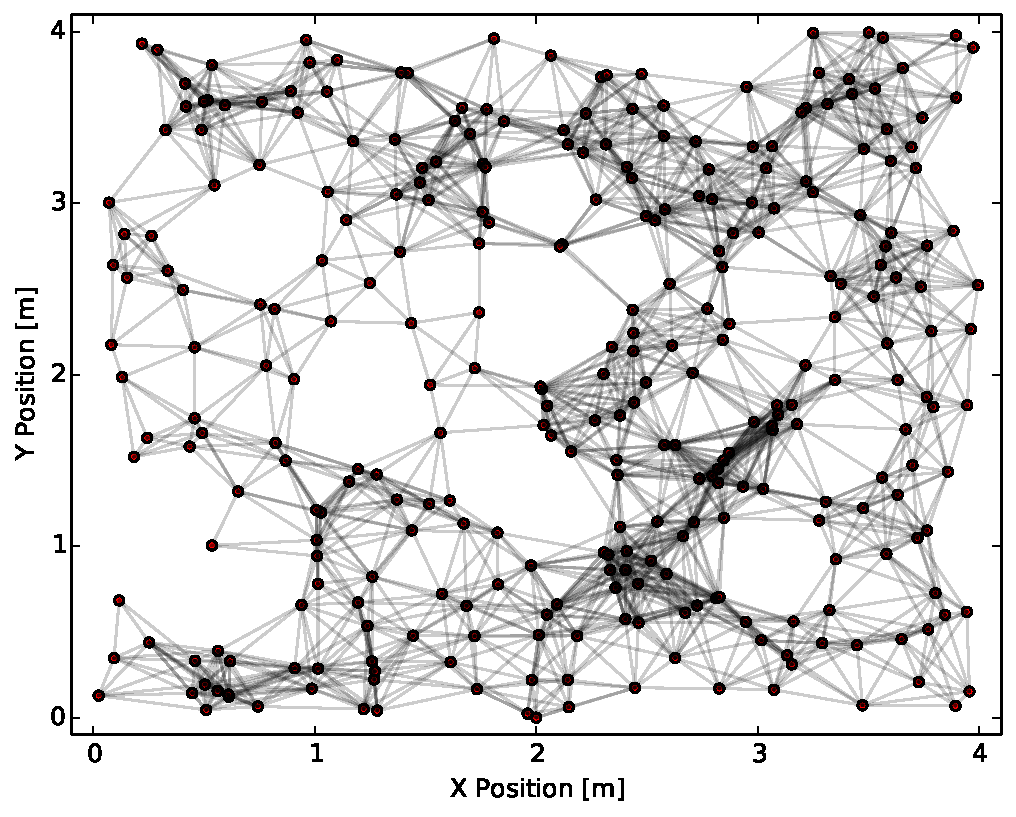
\includegraphics[width=0.8\linewidth]{figs/roadmap}

    \caption{An example of a probabilistic roadmap generated in free space
    without the presence of obstacles. The nodes are represented by the circles
and the red line as the edges between the nodes.}

    \label{fig:prm}
\end{figure}

\subsection{Searching the Graph}

To search the generated two dimensional probabilistic roadmap in space-time, a
novel best first search ($\Acronym{tBestFS}$) algorithm has been developed that
creates a search tree that expands the current node not only in space but also
in time until the current node is within an acceptance radius the goal. This
algorithm works by using priority queue to store to store the expanded nodes.
The priority is based on two things, how many times a two dimensional node in
the probabilistic roadmap has been expanded and the cost to reach the node in
space-time in the queue. A dictionary indexed by the node and mapped to an
integer is used to keep track of how many times the node has been visited. The
cost between two nodes in space-time, $(i, t)$ and $(j, t')$ is defined by the
line integral from $i$ to $j$ over the exponential of the cost distribution $P$
for the time interval $[t_0, t_m]$ and set of dynamic obstacles $A$. This
function uses the exponential of the cost distribution in order to emphasize
higher costs along the path. This is formally shown in Eq.~\ref{eq:cost}.

% Graph cost function

\begin{align}
    C(i, j, t_0, t_m, A) &= \int^1_0 \exp{\Big(
        P(x(\lambda), y(\lambda), t_0, t_m, A) + 1 \Big)
    } \cdot \sqrt{\Big(\frac{\dif x}{\dif t}\Big)^2
    + \Big(\frac{\dif y}{\dif t}\Big)^2}
    \,\mathrm{d}\lambda \notag \\
    % ----------------------------------------------
    &= \int^1_0 \exp{\Big(
        P(x(\lambda), y(\lambda), t_0, t_m, A) + 1 \Big)
    } \cdot \sqrt{(j_x - i_x)^2 + (j_y - i_y)^2}
    \,\mathrm{d}\lambda \notag \\
    % ----------------------------------------------
    &= \int^1_0 \exp{\Big(
        P(x(\lambda), y(\lambda), t_0, t_m, A) + 1 \Big)
    } \cdot ||i - j|| \,\mathrm{d}\lambda
    \label{eq:cost}
\end{align}

In Eq.~\ref{eq:cost}, $C$ is a function $C: \R^2 \times \R^2 \times (\R^+)^2
\times (\R^+)^2 \times \mathcal{A} \rightarrow \R$ where $\mathcal{A}$ is the
set of all possible sets of dynamic obstacles, and $x(\lambda) = (j_x - i_x)
\cdot \lambda + i_x$ and $y(\lambda) = (j_y - i_y) \cdot \lambda + i_y$ are the
parametric equations of the line from $i$ to $j$.  Eq.~\ref{eq:cost} increases
exponentially as the maximum cost along the line increases and therefore makes
edges with larger maximum costs more costly than edges with lower maximum
costs. To combine the two cost formulations for an edge, $((i, t), (j, t'))$, a
weighted sum is computed that adds the number of times node $j$ has been
visited with the line integral over the cost distribution from $i$ to $j$ for
the given time interval. This total cost function is formally described in
Eq.~\ref{eq:totalcost}.

\begin{equation}
    TC(i, j, t_0, t_m, A, D) = \psi \cdot C(i, j, t_0, t_m, A) +
    \omega \cdot D_j
    \label{eq:totalcost}
\end{equation}

In Eq.~\ref{eq:totalcost}, $\psi$ and $\omega$ are scaling constants. It is
important to incorporate a penalty for returning to a location that has already
been visited even if this penalty is small because the tBestFS algorithm may
choose to only expand nodes in a safe area and thus not reach the goal since
there is not a heuristic to sample nodes closer to the goal in order give
preference to safer paths instead of shorter ones.

Since the algorithm operates in both space and time, the search tree is
expanded at a given node, $i$ at a time $t$, by determining how long it would
take the robot to reach all of the neighbours of $i$ and not only adding each
neighbour of $i$ into the priority queue with its associated cost, but also
adding the time at which the robot would reach each neighbour. This is
accomplished by assuming the robot will travel at a constant speed, $s$,
through the environment which makes it easy to compute how long it would take
the robot to reach a neighbour, $j \in \Function{Neighbours}(i)$. The time it
would take for the robot to reach a neighbour, $j$ from $i$ is $||i - j|| / s$
which would make the robot reach $j$ at time $t + ||i - j|| / s$.  Also, since
the algorithm is also operating in time, the robot is able to stay at the same
location for a given wait time $\delta t$ if it is less costly than moving
forward to any of its neighbours.

The algorithm progresses forward by expanding the best current node in the
priority queue. This is the node that has the smallest combined cost in the
queue.  Once a node, $i$ at time $t$, is expanded and its temporal neighbours
determined, the parent for each of these neighbours is defined as $i$ at time
$t$. By storing the parents of each of the neighbours, it becomes possible to
backtrack from the goal to the starting position once the goal is reached and
construct a path to the goal configuration. The algorithm terminates either
when there are no more nodes in the priority queue or once the node popped out
of the queue is less than a certain distance away from the goal node. Once the
node popped out of the priority queue is within the goal region, the path to
the goal is returned. The algorithm used for searching the graph is described
formally in Algo.~\ref{algo:search}.

% Algorithm to search the graph
\begin{algorithm}[ht]
    \caption{$\Acronym{tBestFS}(V, E, R, A, p, g, T)$}
    % \algorithmicrequire{}
    % \\\algorithmicensure{}
    \label{algo:search}
    \begin{algorithmic}[1]
        \setcounter{ALC@line}{0}
        \vspace*{1mm}
        \STATE $Q \leftarrow \Function{PriorityQueue}()$
        \STATE $D \leftarrow \Function{Dictionary}()$
        \STATE $\mathcal{P} \leftarrow \Function{Dictionary}()$
        \STATE $\Function{Insert}(Q, p, T)$
        \WHILE {$|Q| > 0$}
            \STATE $(q, t) \leftarrow \Function{Pop}(Q)$
            \IF{$||q - g|| \leq R$}
                \RETURN $\Function{BacktrackPath}(p, q, t, \mathcal{P})$
            \ENDIF
            \STATE $S \leftarrow \emptyset$
            \STATE $N \leftarrow \Function{Neighbours}(V, E, q) \cup \{q\}$
            \FORALL {$n \in N$}
                \IF {$q \neq n$}
                    \STATE $t' \leftarrow ||q - n|| / s + t$
                \ELSE
                    \STATE $t' \leftarrow t + \delta t$
                \ENDIF
                \STATE $\mathcal{P}_{(n, t')} \leftarrow (q, t)$
                \STATE $c \leftarrow \psi \cdot C(q, n, t, t', A) + \omega
                    \cdot D_{n}$
                \STATE $D_{n} \leftarrow D_{n} + 1$
                \STATE $Q \leftarrow \Function{Insert}(Q, (n, t'), c)$
            \ENDFOR
        \ENDWHILE
    \end{algorithmic}
\end{algorithm}

From the algorithm in Algo.~\ref{algo:search}, it is evident that picking a
good wait time, $\delta t$, is important for generating safe paths through the
environment. Having a large value for $\delta t$ can lead to very suboptimal
paths because even though staying in the same position for a given period of
time may be safer than moving to any of the neighbours, staying there for too
long could lead the planner to miss safer viable paths. For instance, say the
planner has expanded a node, $i$ at time $t$ and $TC(i, i, t, t + \delta t, A,
D) < TC(i, j, t, t + ||i - j|| / s, A, D)$ for all $j \in
\Function{Neighbours}(i)$. There may be a neighbour $j$ and some time $t'$ such
that $t < t' < t + \delta t$ where $TC(i, j, t, t', A, D) < TC(i, i, t, t +
\delta t, A, D)$. Moving the robot to node $j$ at time $t'$ from $i$ at time
$t$ would lead to a safer path than staying at node $i$ until time $t + \delta
t$. This is why it is important for the safety of the generated paths to use a
small value for $\delta t$ in order to not miss sampling safe paths. By using a
smaller value for $\delta t$, the chance that a safer path would be missed
decreases, but the number of nodes in the search tree would increase.

Fig.~\ref{fig:tree} shows how the search tree for $\Acronym{tBestFS}$ is being
built in space-time as the algorithm progresses. The sequence for this figure
is left to right, up to down. The last plot in the Fig.~\ref{fig:tree} also
shows the path in red that was returned by $\Acronym{tBestFS}$.
Fig.~\ref{fig:ex_agents} shows how the dynamic obstacle cost distribution
changes over time for the search tree in Fig.~\ref{fig:tree}. In
Fig.~\ref{fig:tree}, the tree is being expanded into areas that have low cost
in space-time and that is why the tree is being expanded on the left of the
scene. It is evident that the tree is essentially moving around the dynamic
obstacles when they are all near each other on the right side of the scene.

\begin{figure}[h!]
    \centering
    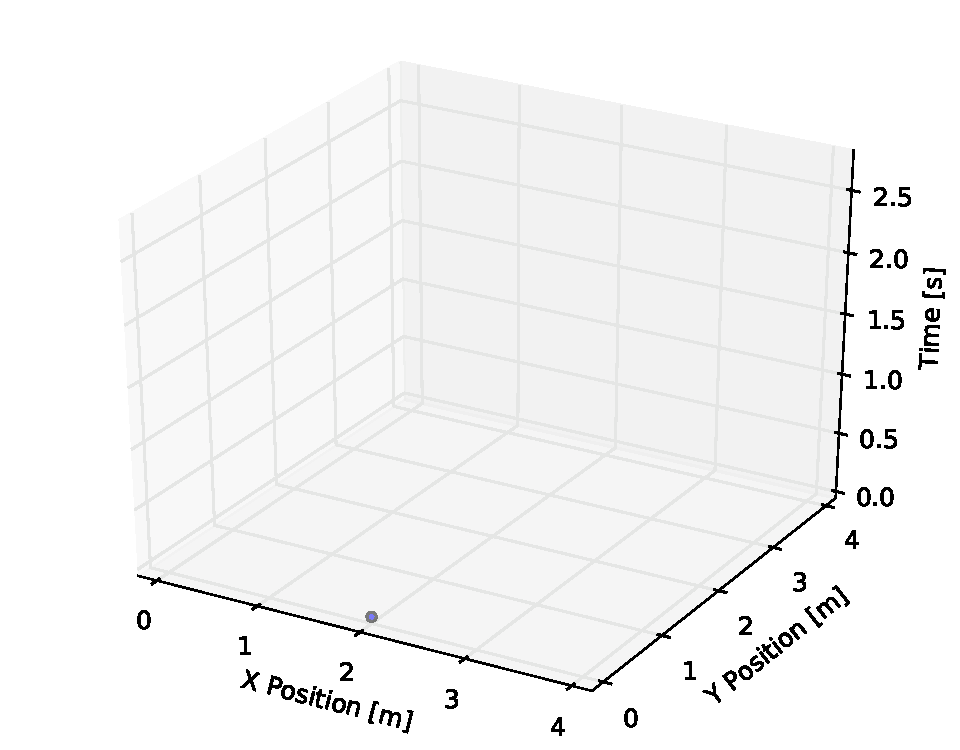
\includegraphics[width=0.32\linewidth]{figs/tree_0}
    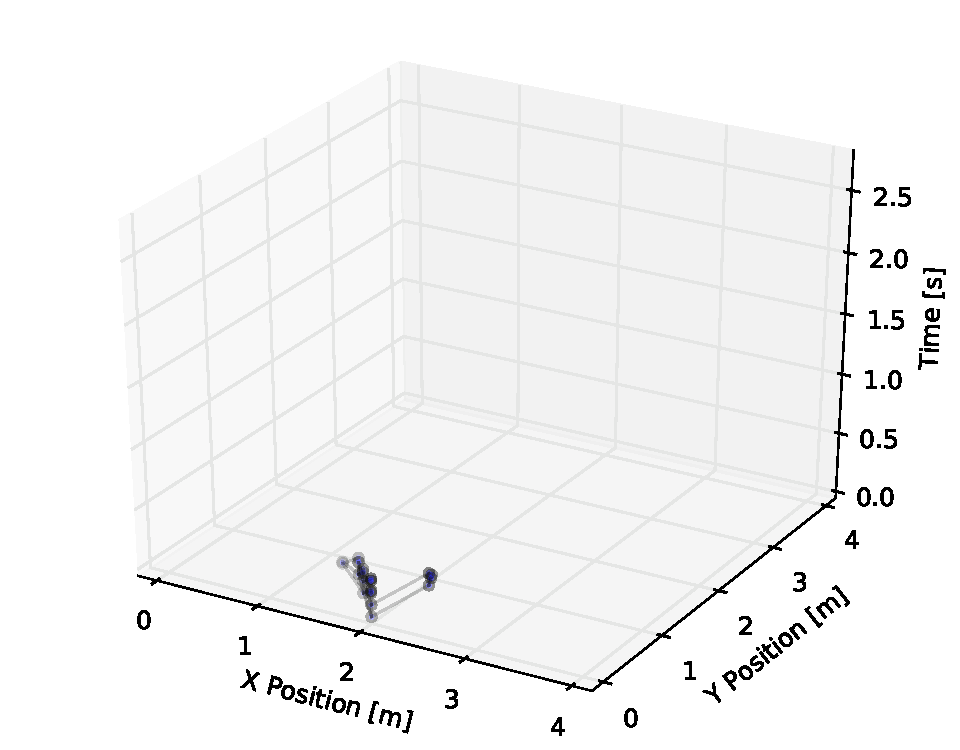
\includegraphics[width=0.32\linewidth]{figs/tree_1}
    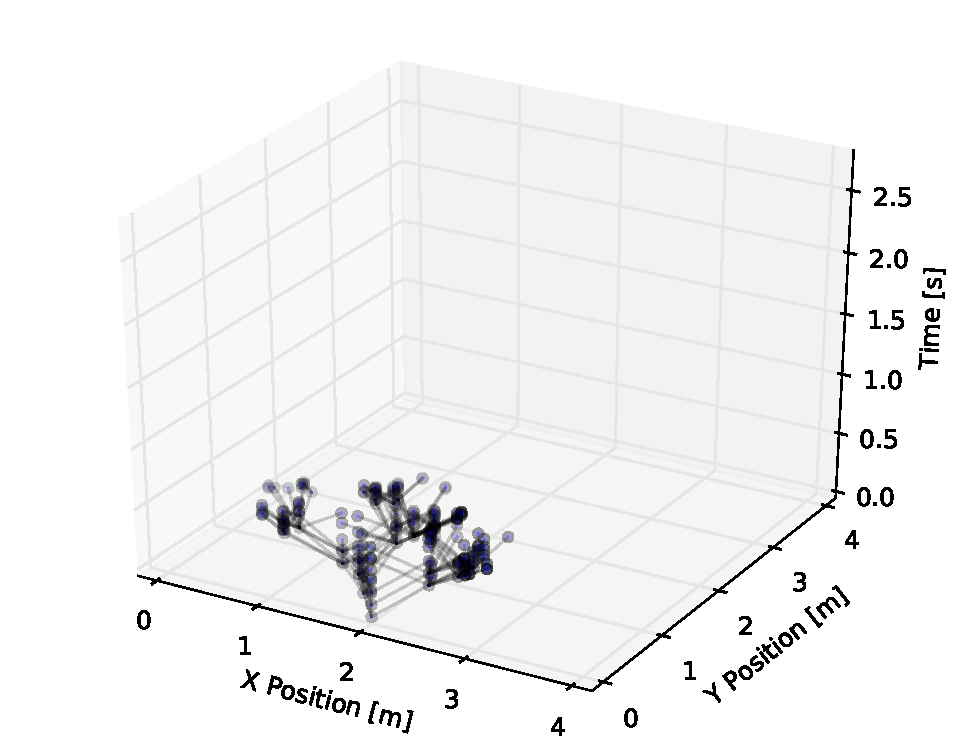
\includegraphics[width=0.32\linewidth]{figs/tree_2} \\
    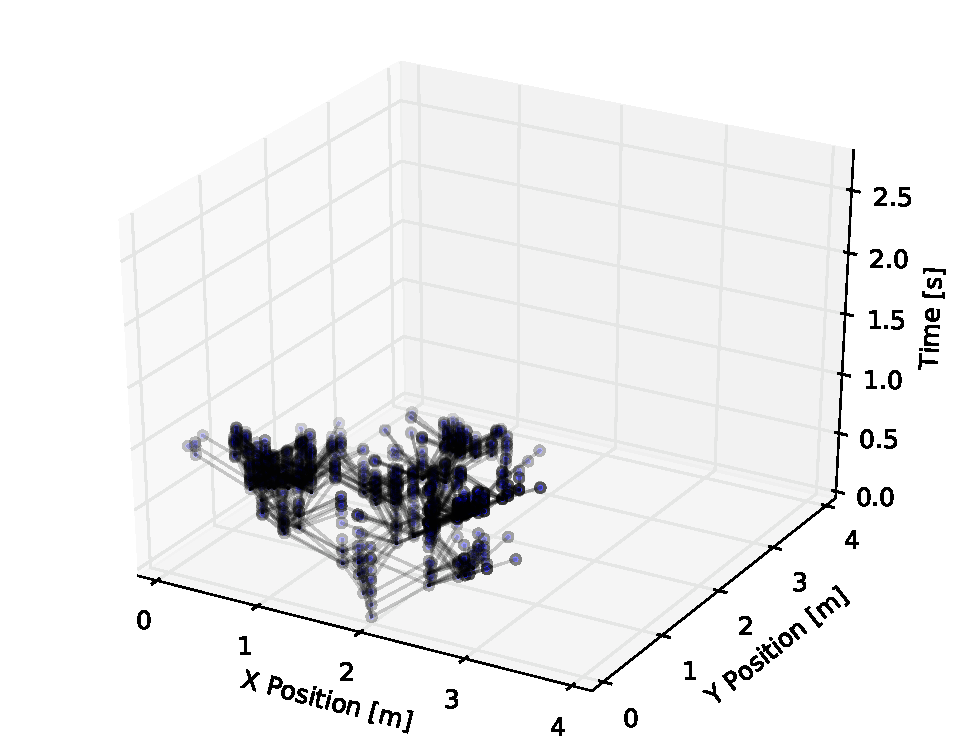
\includegraphics[width=0.32\linewidth]{figs/tree_3}
    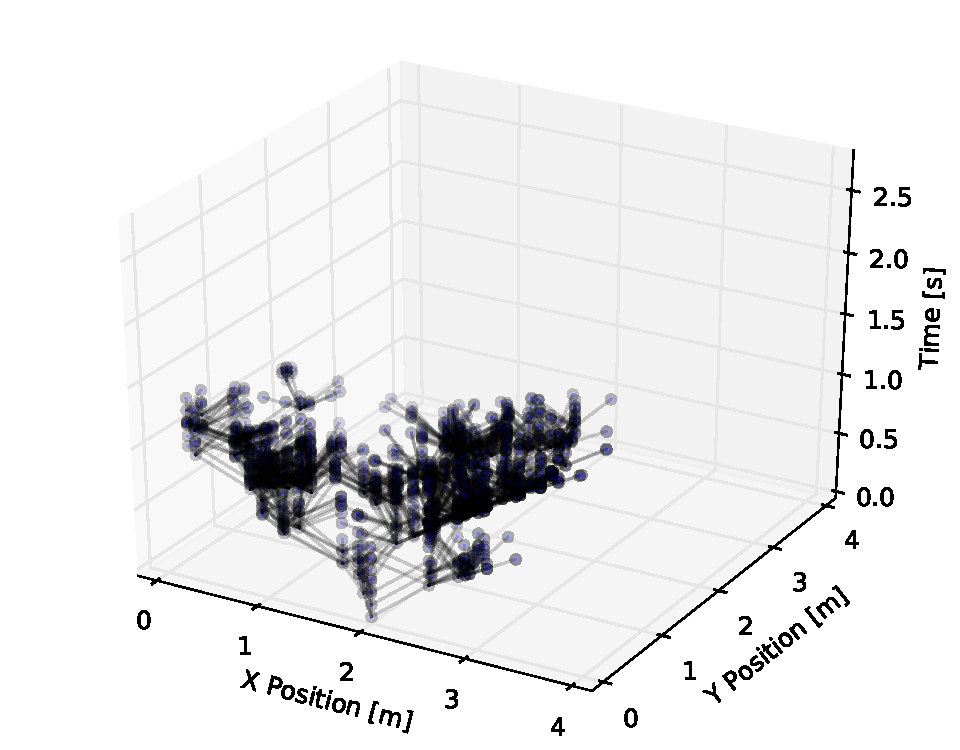
\includegraphics[width=0.32\linewidth]{figs/tree_4}
    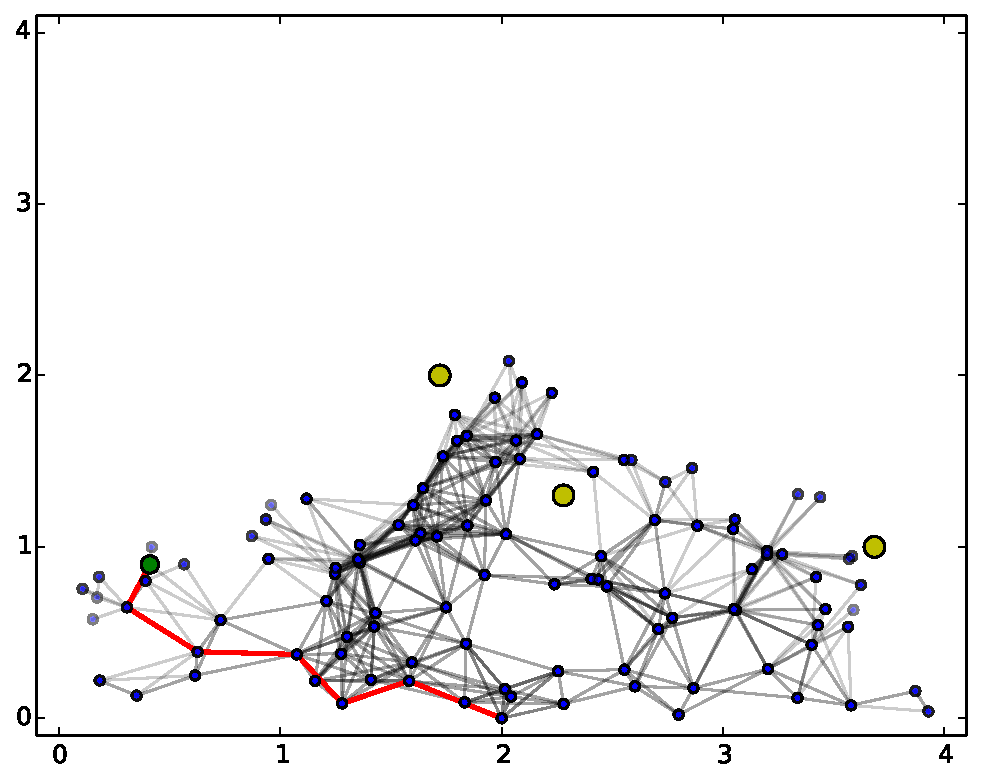
\includegraphics[width=0.32\linewidth]{figs/tree_5} \\
    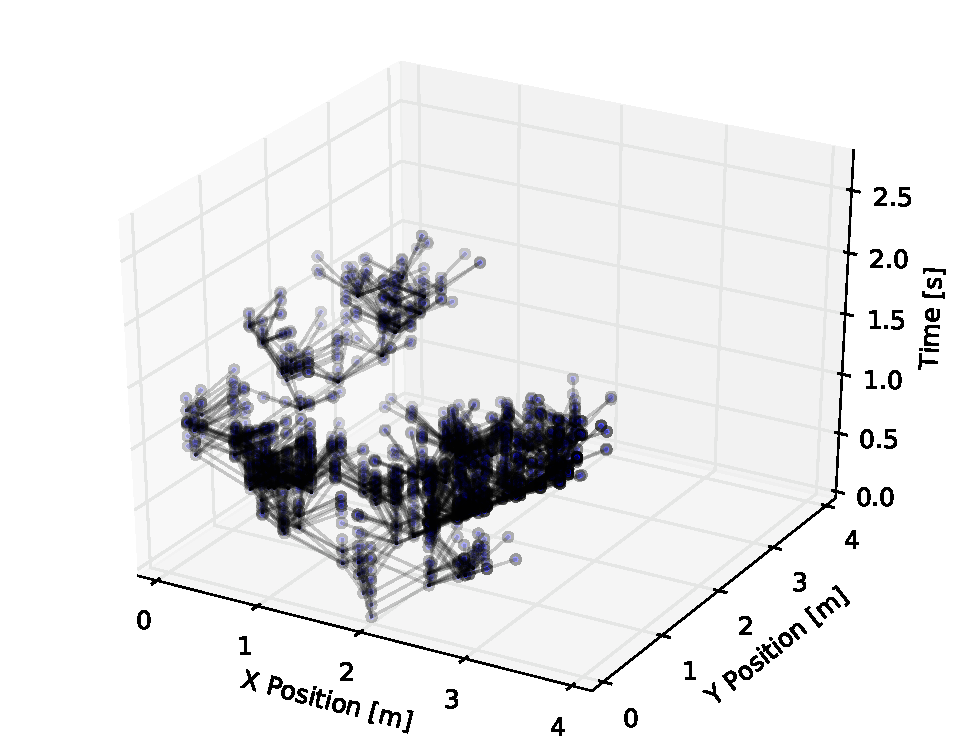
\includegraphics[width=0.32\linewidth]{figs/tree_6}
    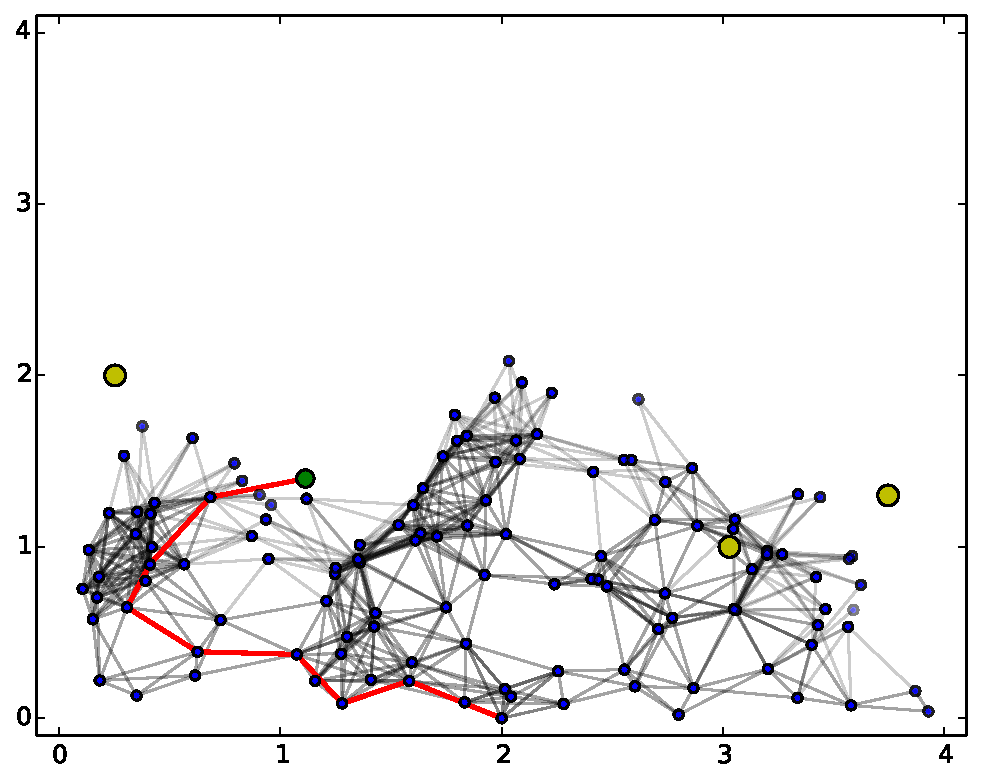
\includegraphics[width=0.32\linewidth]{figs/tree_7}
    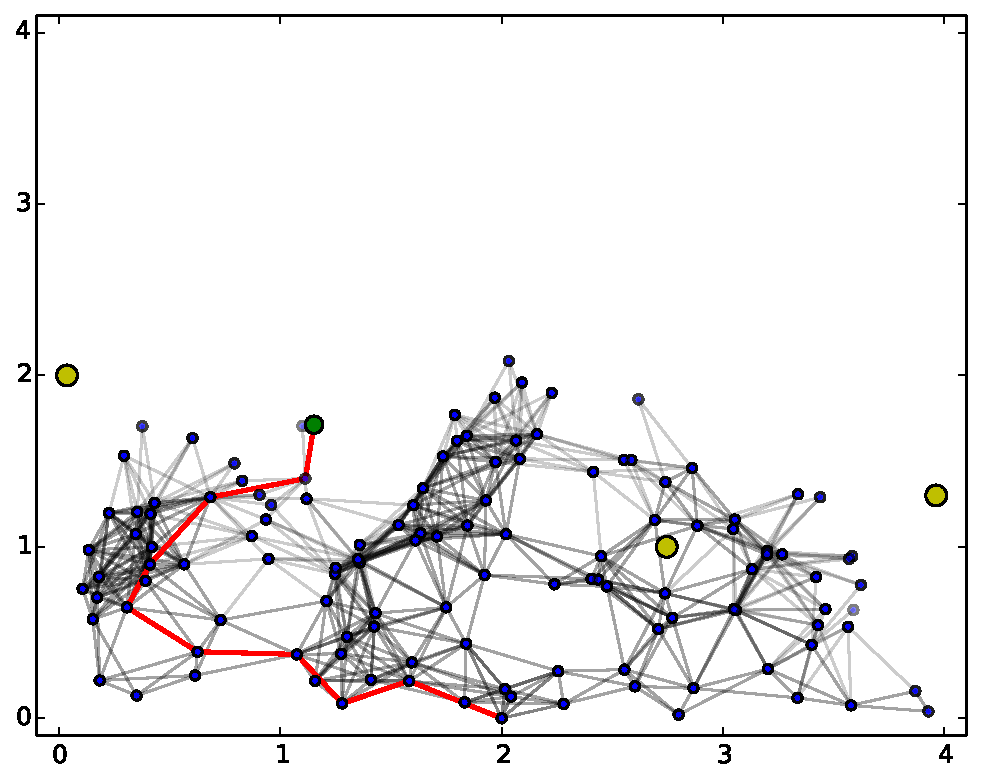
\includegraphics[width=0.32\linewidth]{figs/tree_8}

    \caption{A depiction of the search tree generation for a given
    probabilistic roadmap. The $x$ and $y$ axes represent the $x$ and $y$
location of the node, and the vertical axis represents time. The sequence
progress from left to right, up to down. The final image in sequence also shows
the path taken by the robot in red.}

    \label{fig:tree}
\end{figure}

\begin{figure}[h!]
    \centering
    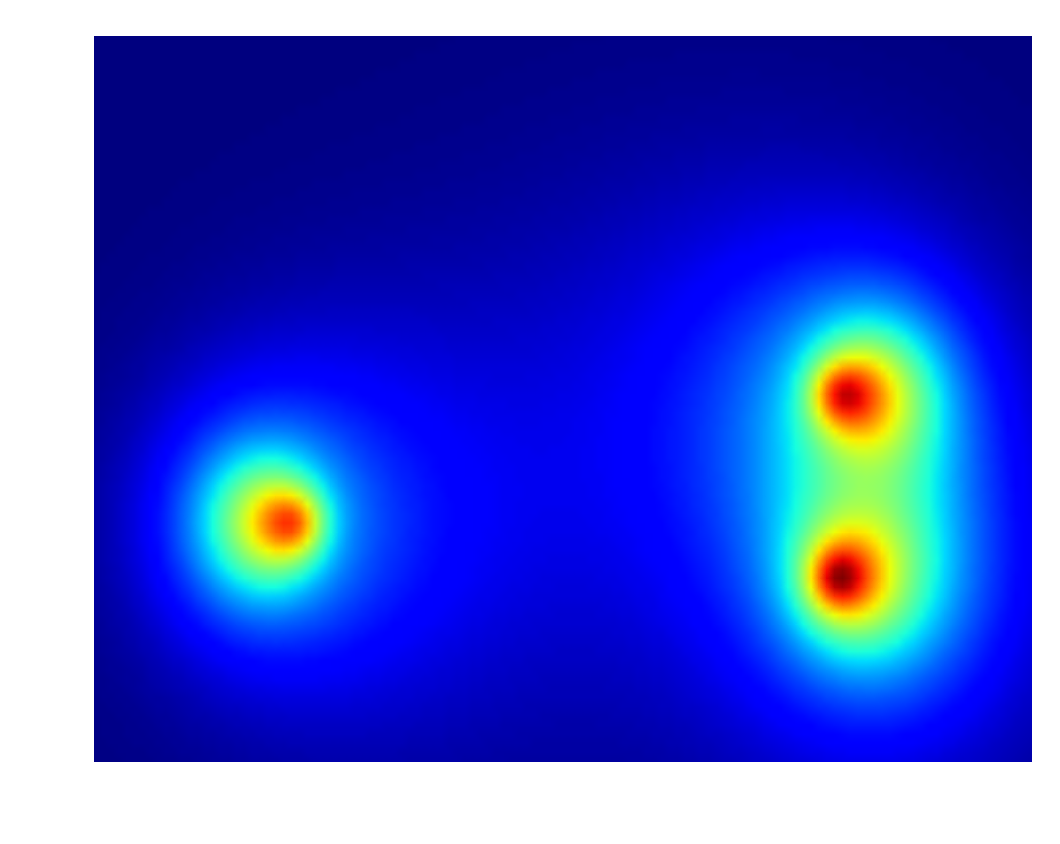
\includegraphics[width=0.32\linewidth]{figs/ex_agent_0}
    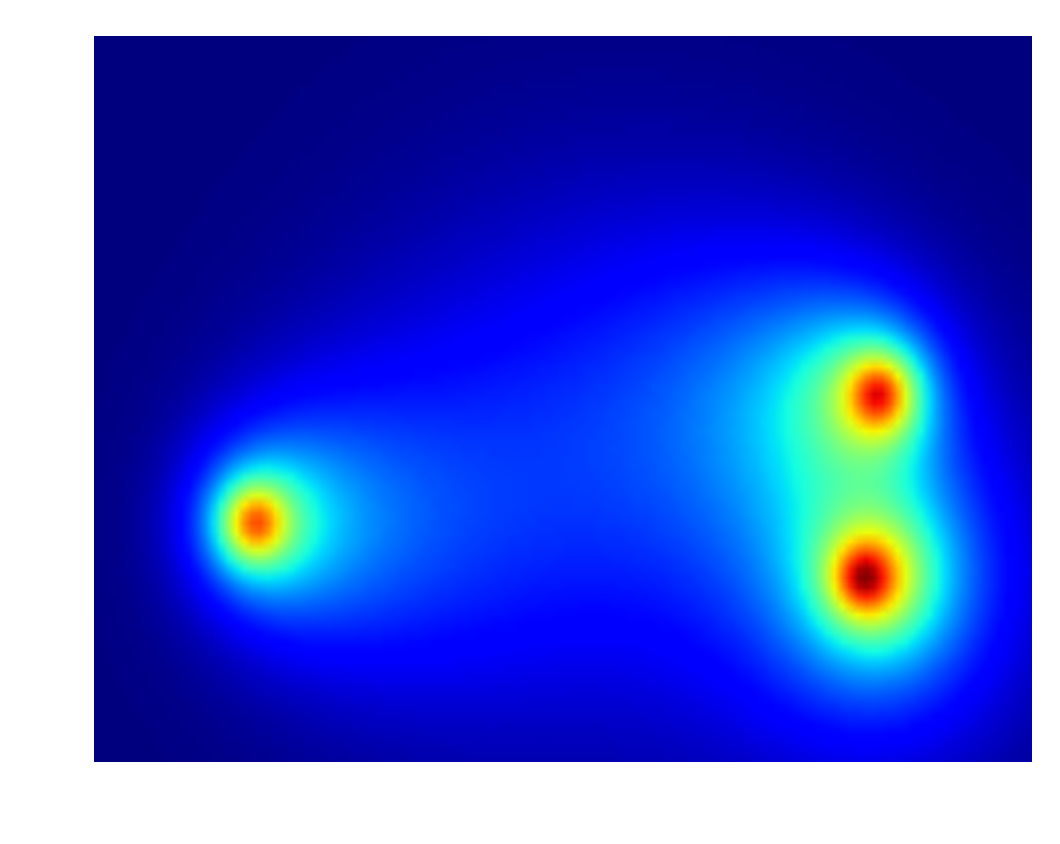
\includegraphics[width=0.32\linewidth]{figs/ex_agent_1}
    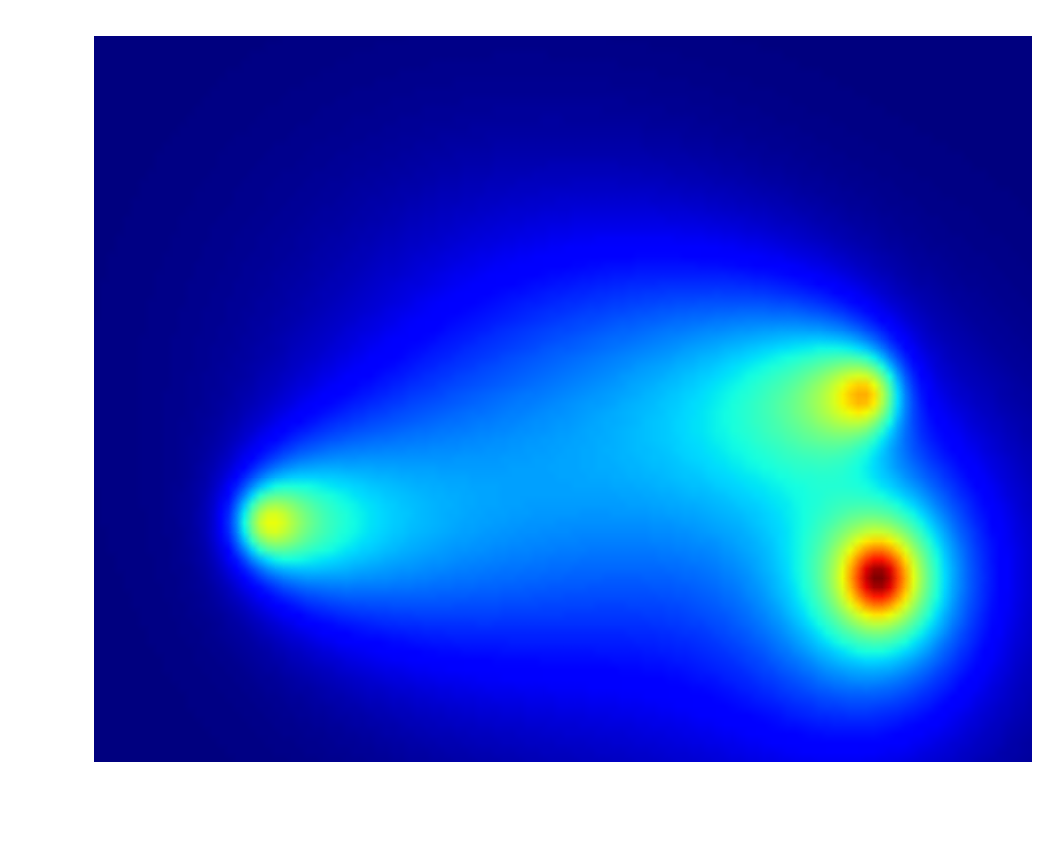
\includegraphics[width=0.32\linewidth]{figs/ex_agent_2} \\
    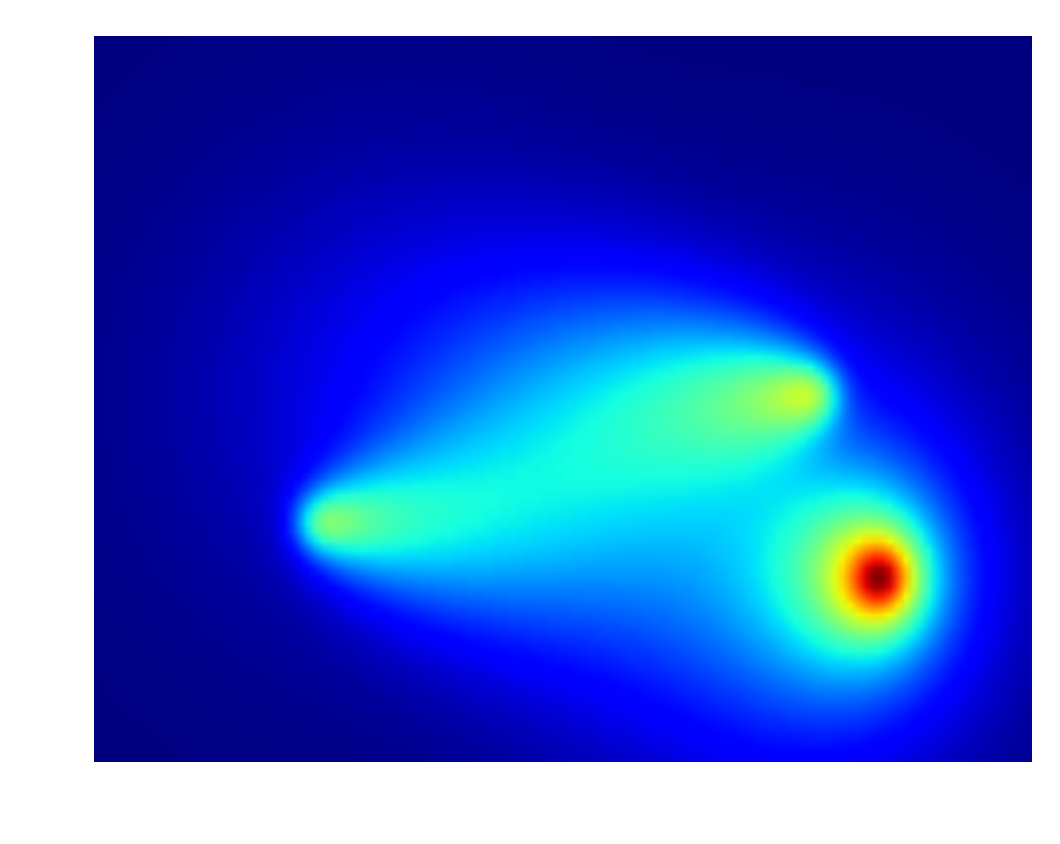
\includegraphics[width=0.32\linewidth]{figs/ex_agent_3}
    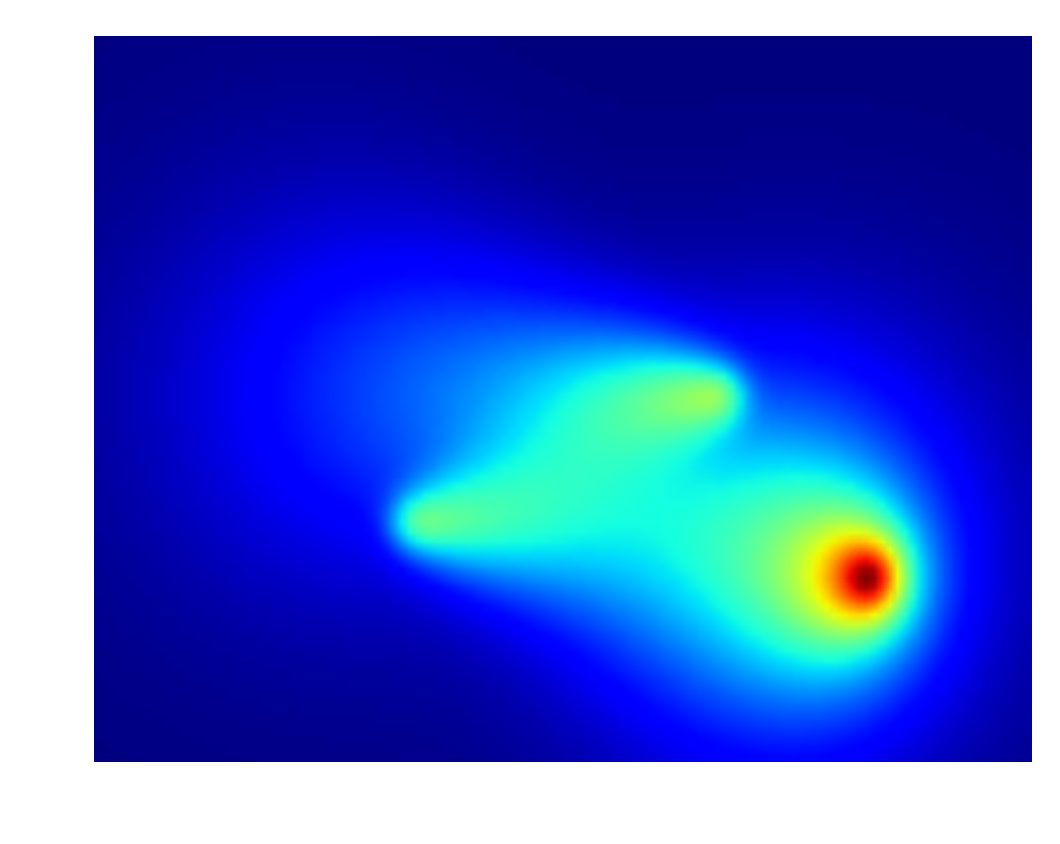
\includegraphics[width=0.32\linewidth]{figs/ex_agent_4}
    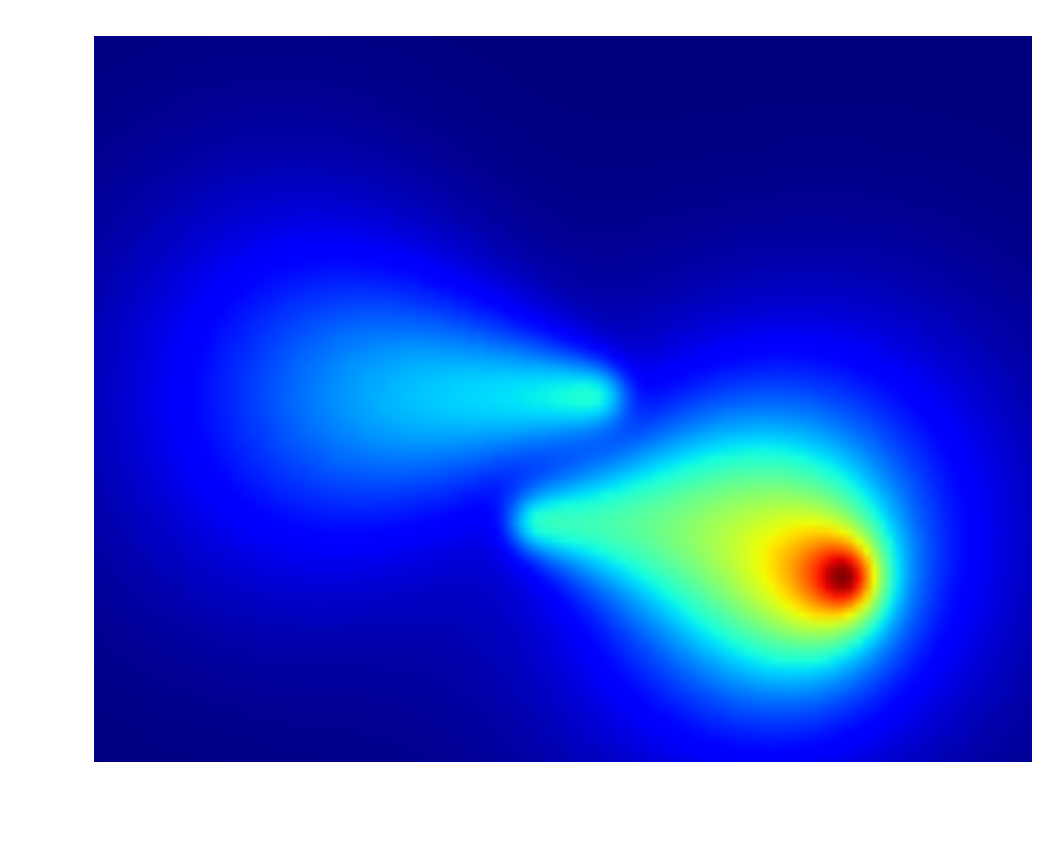
\includegraphics[width=0.32\linewidth]{figs/ex_agent_5} \\
    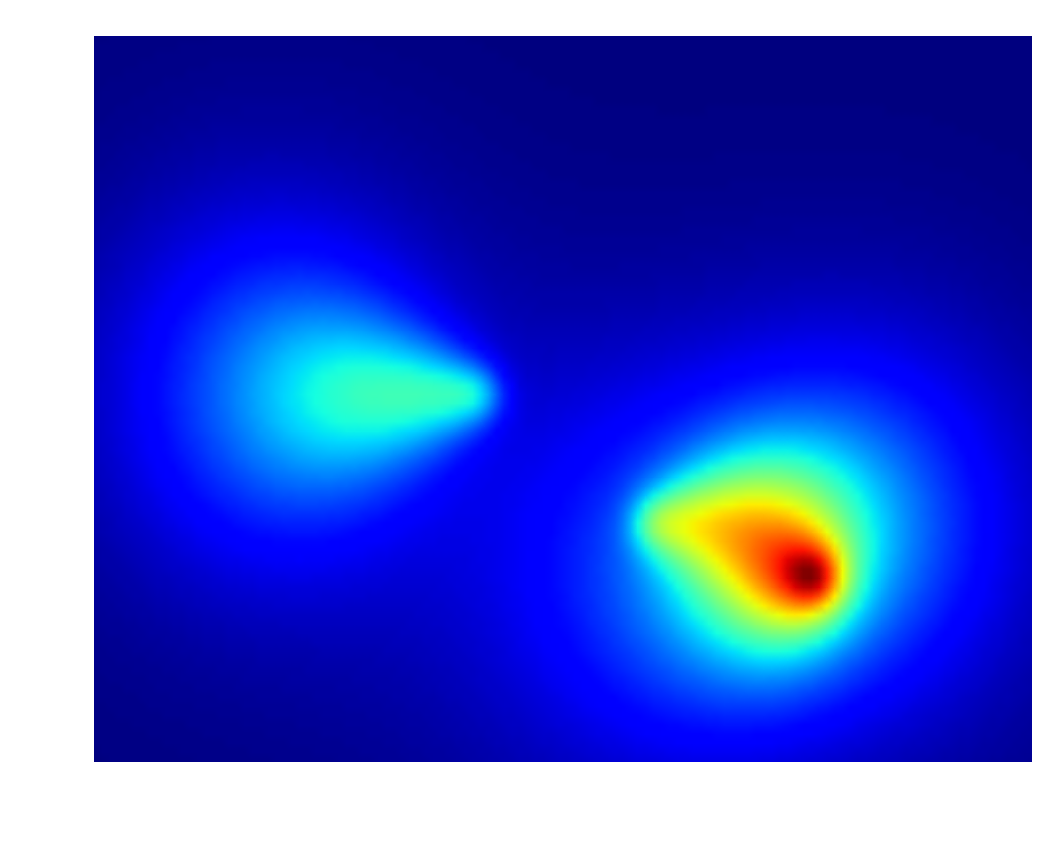
\includegraphics[width=0.32\linewidth]{figs/ex_agent_6}
    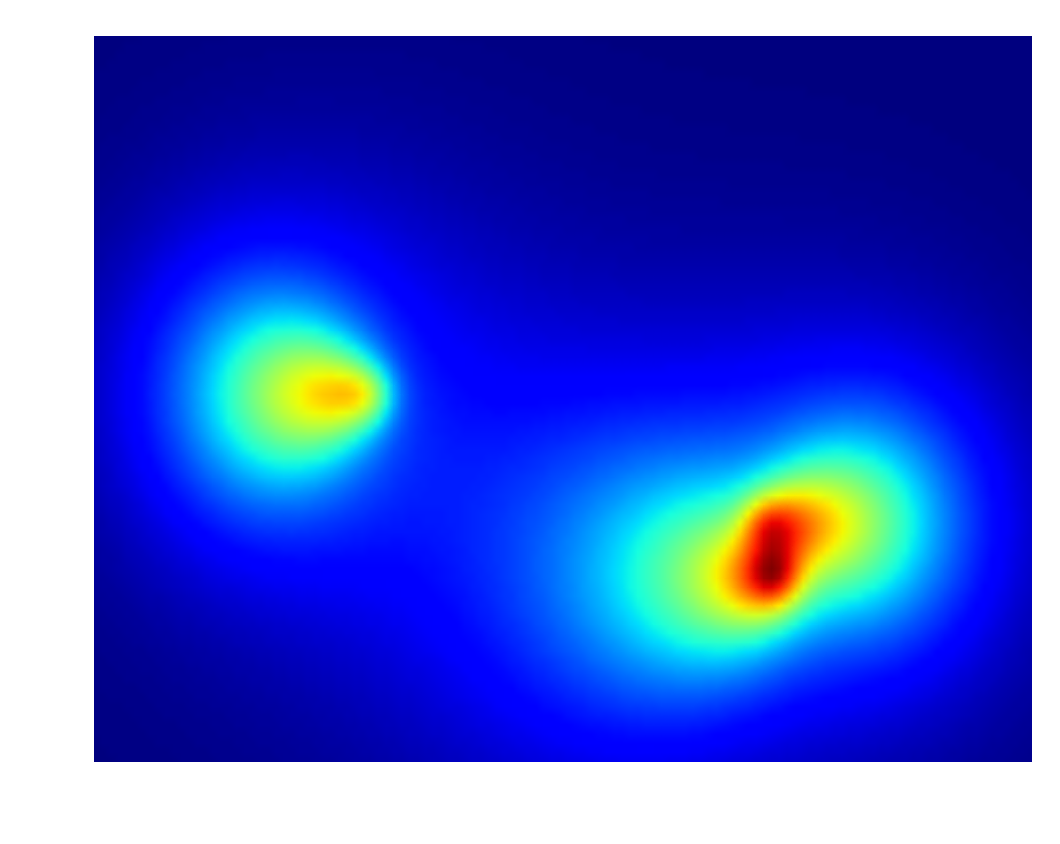
\includegraphics[width=0.32\linewidth]{figs/ex_agent_7}
    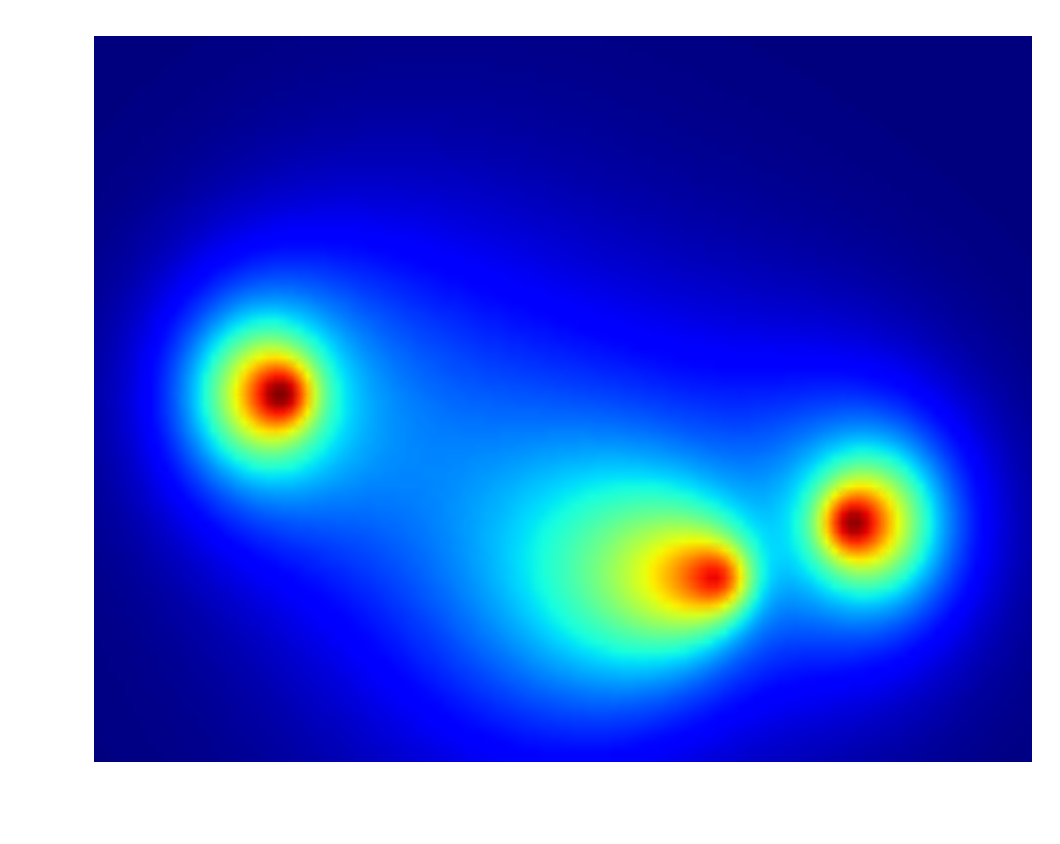
\includegraphics[width=0.32\linewidth]{figs/ex_agent_8}

    \caption{A sequence of images showing the progression of the cost
    distribution for the set of dynamic obstacles over time used for the search
tree shown in Fig.~\ref{fig:tree}. The sequence progresses from left to right,
up to down.}

    \label{fig:ex_agents}
\end{figure}


% % Given a parent dictionary, this returns the backtracked path
% \begin{algorithm}[ht]
%     \caption{$\Function{BacktrackPath}(p, g, t, \mathcal{P})$}
%     % \algorithmicrequire{}
%     % \\\algorithmicensure{}
%     \label{algo:backtrack}
%     \begin{algorithmic}[1]
%         \setcounter{ALC@line}{0}
%         \vspace*{1mm}
%         \STATE $(q, t') \leftarrow (g, t)$
%         \STATE $S \leftarrow \Function{Stack}()$
%         \WHILE {$\mathcal{P}_{(q, t')} \neq (p, 0)$}
%             \STATE $S \leftarrow \Function{Push}(S, (q, t'))$
%             \STATE $(q, t') \leftarrow \mathcal{P}_{(q, t')}$
%         \ENDWHILE
%         \STATE $S \leftarrow \Function{Push}(S, (p, 0))$
%         \RETURN $S$
%     \end{algorithmic}
% \end{algorithm}

\subsubsection{Completeness}

It is important to prove certain properties about the completeness of the
$\Acronym{tBestFS}$ algorithm in order to guarantee that the algorithm will
always return a path in a finite amount of time. For the completeness proof it
is first important to prove properties about the bounds of the two functions
that comprise the total cost function for an edge. The proof for completeness
rests on the fact that the added penalty of returning to a node will be
monotonically increasing as the number of times the node has been visited
increases and that the cost of an edge is strictly finite for all acceptable
parameters. The proof uses these properties to show that in a finite amount of
time, it will be more favourable to expand towards the goal node than to stay
in the same location.

\begin{lemma}

    \label{theorem:increasing}

    The added penalty of returning to a node in the probabilistic roadmap is
    monotonically increasing.

\end{lemma}

\begin{proof}

    Since the added penalty for returning to a node increases by one each time
    the node is visited, as the number of times it has been revisited increases
    to infinity, so does the added penalty.

\end{proof}

\begin{corollary}

    The total cost, $TC$, is a monotonically increasing function.

\end{corollary}

The second property of the functions that make up the edge cost is shown in
Lemma~\ref{theorem:capped} which describes that the cost function, $C$ will
always have a value less than infinity for all permissible parameters.

\begin{lemma}

    \label{theorem:capped}

    The cost for any $(m, n) \in E$ for a time interval $[t, t']$ such that $t'
    - t < \infty$ is strictly less than infinity and $0 < t < t'$.

\end{lemma}

\begin{proof}

    The function, $C$, can only increase to infinity if the two nodes on the
    edge are an infinite distance apart or if the cost distribution in
    Eq.~\ref{eq:singleprob}, $P$, increases towards infinity. For the former,
    two nodes cannot be an infinite distance apart because the connection
    distance, $d$, is set to be strictly less than infinity and because the
    $\forall i, j \in V : ||i - j|| \leq \sqrt{w^2 + h^2}$ where $0 < w <
    \infty$ and $0 < h < \infty$ are the width and height of the scene
    respectively. Therefore $C$ cannot tend to infinity because of the distance
    between nodes since no two nodes are an infinite distance away. For the
    latter, $P$ can only tend to infinity if the normal distribution,
    $\mathcal{N}$ reaches infinity. This is only possible if the variance
    approaches 0. However the variance cannot reach $0$ in case because the
    constant $\beta$ is always greater than zero. Therefore it is impossible
    for the cost along an edge, $C$, to tend towards infinity.

\end{proof}

Using Lemmas~\ref{theorem:increasing} and~\ref{theorem:capped}, a proof can be
constructed for Theorem~\ref{theorem:completeness} which states that
$\Acronym{tBestFS}$ is complete and will always return a path.

\begin{theorem}

    \label{theorem:completeness}

    $\Acronym{tBestFS}$ will always return a path in a finite amount of time.

\end{theorem}

\begin{proof}

    First, it is important for the proof to note that the penalty for returning
    to a previously visited location increases monotonically to infinity as the
    number of visits for a particular node approaches infinity. Also, the cost
    function, $C$, is bounded strictly below infinity for all possible
    parameters. Now assume the pathological case where $\forall (m, n)
    \in E, \forall i \in \Function{Neighbours}(g) : C(i, g, t, t', A) > C(m, n,
    t, t', A)$ for all time intervals $[t, t']$ and where $g$ is the goal node
    in the probabilistic roadmap. This means that the cost to reach the goal
    will be larger than any edge cost at any time in the graph.  Therefore,
    without the added penalty for returning to a previously visited location,
    the goal will never be popped out of the priority queue for expansion.
    However, since there is a penalty for returning to the same geometrical
    location, as the algorithm progresses, $\forall (m, n)
    \in E, \forall i \in \Function{Neighbours}(g) : TC(i, g, t, t', A, D) <
    TC(m, n, t, t', A, D)$ because each node in the probabilistic roadmap
    except the goal node would have been expanded one or more times, thus
    increasing the added penalty. Since the goal node has not been expanded,
    its total cost would only be the value for $C$ and since $C$ is bounded
    below infinity and the added penalty increases monotonically towards
    infinity, all edges to the goal node would have a lower cost than any edge
    to any other node and thus the goal would be expanded. If the goal is
    expanded, a path to the goal would be returned. The path is returned in a
    finite amount of time because the number of nodes in the graph is finite.

\end{proof}

\subsection{Replanning}

In order to generate safe paths in uncertain, stochastic environments, the
planner is not able to simply provide an \emph{a priori} plan from the
$\Acronym{tBestFS}$ algorithm. It is necessary for the planner to generate new
paths from the current configuration of the robot as it progresses through the
environment if the actual trajectory of a dynamic obstacle deviates too much
from its predicted trajectory. This planning occurs in real-time during the
execution of the path in the environment. This framework for regenerating paths
is called \emph{replanning}. Replanning for this work occurs once the model of
movement for a given dynamic obstacle can no longer predict within an
acceptable error the actual position of the dynamic obstacle. When replanning,
the same probabilistic roadmap is used and the connectivity of the environment
is not resampled.

Replanning works by first generating a preliminary path through the environment
using the $\Acronym{tBestFS}$ algorithm. The robot will then follow this path
by moving at its prescribed constant speed, $s$, in a straight line from node
to node in the path. Once it reaches a node, $i$ at time $t$ in the path, the
robot checks whether the actual locations of the obstacles either sensed by the
robot or by an external system differ more than an acceptable amount, $\delta$,
from the predicted locations of the dynamic obstacles at time $t$ i.e.

$$\bigvee_{a \in A} ||\tilde{\zeta_a}(t) - \zeta_a(t)|| > \delta$$

Where $A$ is the set of dynamic obstacles. If this proposition is true, there
is substantial deviation in the obstacle positions, the planner will update the
value of the dynamic variables, $T$ and $\xi$ for the obstacles which are used
for predicting their trajectories to $t$ and $\tilde{\zeta_a}(t)$ respectively.
These variables are part of the 5-tuple defining the dynamic obstacles which is
described in Sec.~\ref{sec:def}. Once these variables are updated, the graph is
searched using the $\Acronym{tBestFS}$ algorithm starting from the current
position of the robot, $i$ with a starting time of $t$. It is also important to
note that the same dictionary used for storing how many times a node has been
visited when researching the graph. The actual path of the robot is a union of
the past locations of the robot based on the partial paths generated whilst
traversing the environment. Algo.~\ref{algo:path} describes the processes of
replanning due to the deviations in the obstacle locations and is the main
entry point for the Dodger algorithm.

% Main algorithm to get the path
\begin{algorithm}[ht]
    \caption{$\Function{Dodger}(n, d, w, h, \delta, p, g, O, A, R)$}
    \algorithmicrequire{
        \\$n$: Maximum number of samples for the roadmap
        \\$d$: Maximum distance between neighbouring nodes in the roadmap
        \\$w$: Width of the scene
        \\$h$: Height of the scene
    }
    \\\algorithmicensure{}
    \label{algo:path}
    \begin{algorithmic}[1]
        \setcounter{ALC@line}{0}
        \STATE $(V, E) \leftarrow \Function{Roadmap}(n, d, w, h, O)$
        \STATE $\Pi \leftarrow \emptyset$
        \STATE $q \leftarrow p$
        \STATE $t \leftarrow 0$
        \WHILE {$||\Function{Back}(\Pi) - g||_2 > R$}
            \STATE $\pi \leftarrow \Function{SearchGraph}(V, E, R, A, q, g, t)$
            \FORALL {$(i, t') \in \pi$}
                \STATE $\Pi \leftarrow \Pi \cup \{i\}$
                \FORALL {$a \in A$}
                    \STATE $\Function{Step}(a)$
                \ENDFOR
                \IF {$\bigvee_{a \in A} ||\tilde{\zeta_a}(t') -
                    \zeta_a(t')|| > \delta$}
                    \FORALL {$a \in A$}
                        \STATE $T_a \leftarrow t'$
                        \STATE $\xi_a \leftarrow \tilde{\zeta_a}(t')$
                    \ENDFOR
                    \STATE $q \leftarrow i$
                    \STATE $t \leftarrow t'$
                    \STATE $\textbf{break}$
                \ENDIF
            \ENDFOR
        \ENDWHILE
        \RETURN $\Pi$
    \end{algorithmic}
\end{algorithm}

Replanning is necessary because it allows the planner to redirect the robot to
new, safer paths as the environment changes. This is important because the
initial path generated by the $\Acronym{tBestFS}$ algorithm uses the predicted
motion of the obstacles and assumes they will stay on this predicted trajectory
for the execution of the path. The $\Acronym{tBestFS}$ is able to account for
some uncertainty in the motion of the obstacles as described by the cost
distribution in Sec.~\ref{sec:cost} but this distribution is not able to fully
account for path divergences. By updating the information for the dynamic
obstacles and re-searching the probabilistic roadmap using $\Acronym{tBestFS}$,
safer overall paths can be generated. It is possible to regulate the number of
times the planner will need to replan and thus the safety of the plan by
adjusting the value for $\delta$. The larger the value for $\delta$, the more
the obstacles the will need to diverge from the prescribed trajectories in
order to replan and vice-versa.

\subsubsection{Completeness}

\begin{theorem}

    The robot will always reach the goal in a finite amount of time given the
    proposed replanning scheme outlined in Algo.~\ref{algo:path} for $\delta >
    0$.

\end{theorem}

\begin{proof}



\end{proof}

\subsection{Discussion}

\label{sec:plannerdiscussion}

The final algorithm developed is able to generate low cost paths through the
environment by using the available information about the obstacles' motion. The
planner is able to do this by searching through space-time over a two
dimensional graph using the $\Acronym{tBestFS}$ algorithm which uses the cost
distribution described in Sec.~\ref{sec:cost} to weight the edges of the search
tree. The algorithm is also able to adapt and create new plans through the
environment when its' prediction of the obstacles' motion is no longer able to
accurately determine where the obstacles are going to be in future. This
replanning stage of the algorithm allows it to be used in real-time in
stochastic dynamic environments. This mimics the reactive behaviour of
potential fields, with the added benefit of provable completeness and not being
a solely reactive planner. Likewise, the replanning ability allows the
information given to the planner about the motion of the obstacles not to be
perfect. Even if the equations of motion that the motion prediction system
provides in now way describe the actual motion of the obstacles, the algorithm
will simply replan at every time step and instead of using the cost
distributions to determine paths through the environment, the planner will
simply move to the next best node in the probabilistic roadmap. This means that
the algorithm is able to continuously plan through stochastic dynamic
environments utilizing the available information to move the robot to the goal.

\end{document}
